%%%%%%%%%%%%%%%%%%%%%%%%%%%%%%%%%%%%%%%%%%%%%%%%%%%%%%%%%%%%%%%
%% CDE THESIS TEMPLATE

% Use this template to produce a standard thesis that meets the CDE master requirements for submission
%
% Originally by Keith A. Gillow (gillow@maths.ox.ac.uk), 1997
% Modified by Sam Evans (sam@samuelevansresearch.org), 2007
% Modified by John McManigle (john@oxfordechoes.com), 2015
% Modified by Ulrik Lyngs (ulrik.lyngs@cs.ox.ac.uk), 2018-, for use with R Markdown
% Modified by Cesar Aybar (csaybar@gmail.com), 2022-, according to CDE format.

% Ulrik Lyngs, 25 Nov 2018: Following John McManigle, broad permissions are granted to use, modify, and distribute this software
% as specified in the MIT License included in this distribution's LICENSE file.
%
% John commented this file extensively, so read through to see how to use the various options.  Remember that in LaTeX,
% any line starting with a % is NOT executed.  Several places below, you have a choice of which line to use
% out of multiple options (eg draft vs final, for PDF vs for binding, etc.)  When you pick one, add a % to the beginning of
% the lines you don't want.


%%%%% PAGE LAYOUT
% The most common choices should be below.  You can also do other things, like replacing "a4paper" with "letterpaper", etc.

% This one formats for two-sided binding (ie left and right pages have mirror margins; blank pages inserted where needed):
%\documentclass[a4paper,twoside]{templates/ociamthesis}
% This one formats for one-sided binding (ie left margin > right margin; no extra blank pages):
%\documentclass[a4paper]{ociamthesis}
% This one formats for PDF output (ie equal margins, no extra blank pages):
%\documentclass[a4paper,nobind]{templates/ociamthesis}

% As you can see from the uncommented line below, oxforddown template uses the a4paper size, 
% and passes in the binding option from the YAML header in index.Rmd:
\documentclass[a4paper, nobind]{templates/cdethesis}


%%%%% ADDING LATEX PACKAGES
% add hyperref package with options from YAML %
\usepackage[pdfpagelabels]{hyperref}
% change the default coloring of links to something sensible
\usepackage{xcolor}

\definecolor{mylinkcolor}{RGB}{0,0,139}
\definecolor{myurlcolor}{RGB}{0,0,139}
\definecolor{mycitecolor}{RGB}{0,33,71}

\hypersetup{
  hidelinks,
  colorlinks,
  linktocpage=true,
  linkcolor=mylinkcolor,
  urlcolor=myurlcolor,
  citecolor=mycitecolor
}



% add float package to allow manual control of figure positioning %
\usepackage{float}

% enable strikethrough
\usepackage[normalem]{ulem}

% use soul package for correction highlighting
\usepackage{color, soul}
\definecolor{correctioncolor}{HTML}{CCCCFF}
\sethlcolor{correctioncolor}
\newcommand{\ctext}[3][RGB]{%
  \begingroup
  \definecolor{hlcolor}{#1}{#2}\sethlcolor{hlcolor}%
  \hl{#3}%
  \endgroup
}
\soulregister\ref7
\soulregister\cite7
\soulregister\autocite7
\soulregister\textcite7
\soulregister\pageref7

%%%%% FIXING / ADDING THINGS THAT'S SPECIAL TO R MARKDOWN'S USE OF LATEX TEMPLATES
% pandoc puts lists in 'tightlist' command when no space between bullet points in Rmd file,
% so we add this command to the template
\providecommand{\tightlist}{%
  \setlength{\itemsep}{0pt}\setlength{\parskip}{0pt}}
 
% UL 1 Dec 2018, fix to include code in shaded environments

% User-included things with header_includes or in_header will appear here
% kableExtra packages will appear here if you use library(kableExtra)
\usepackage{booktabs}
\usepackage{longtable}
\usepackage{array}
\usepackage{multirow}
\usepackage{wrapfig}
\usepackage{float}
\usepackage{colortbl}
\usepackage{pdflscape}
\usepackage{tabu}
\usepackage{threeparttable}
\usepackage{threeparttablex}
\usepackage[normalem]{ulem}
\usepackage{makecell}
\usepackage{xcolor}


%UL set section header spacing
\usepackage{titlesec}
% 
\titlespacing\subsubsection{0pt}{24pt plus 4pt minus 2pt}{0pt plus 2pt minus 2pt}


%UL set whitespace around verbatim environments
\usepackage{etoolbox}
\makeatletter
\preto{\@verbatim}{\topsep=0pt \partopsep=0pt }
\makeatother


%%%%%%% PAGE HEADERS AND FOOTERS %%%%%%%%%
\usepackage{fancyhdr}
\setlength{\headheight}{15pt}
\fancyhf{} % clear the header and footers
\pagestyle{fancy}
\renewcommand{\chaptermark}[1]{\markboth{\thechapter. #1}{\thechapter. #1}}
\renewcommand{\sectionmark}[1]{\markright{\thesection. #1}} 
\renewcommand{\headrulewidth}{0pt}

\fancyhead[LO]{\emph{\leftmark}} 
\fancyhead[RE]{\emph{\rightmark}} 

% UL page number position 
\fancyfoot[C]{\emph{\thepage}} %regular pages
\fancypagestyle{plain}{\fancyhf{}\fancyfoot[C]{\emph{\thepage}}} %chapter pages

% JEM fix header on cleared pages for openright
\def\cleardoublepage{\clearpage\if@twoside \ifodd\c@page\else
   \hbox{}
   \fancyfoot[C]{}
   \newpage
   \if@twocolumn\hbox{}\newpage
   \fi
   \fancyhead[LO]{\emph{\leftmark}} 
   \fancyhead[RE]{\emph{\rightmark}} 
   \fi\fi}


%%%%% SELECT YOUR DRAFT OPTIONS
% This adds a "DRAFT" footer to every normal page.  (The first page of each chapter is not a "normal" page.)

% IP feb 2021: option to include line numbers in PDF

% for line wrapping in code blocks
\usepackage{fvextra}
\DefineVerbatimEnvironment{Highlighting}{Verbatim}{breaklines,commandchars=\\\{\}}

% This highlights (in blue) corrections marked with (for words) \mccorrect{blah} or (for whole
% paragraphs) \begin{mccorrection} . . . \end{mccorrection}.  This can be useful for sending a PDF of
% your corrected thesis to your examiners for review.  Turn it off, and the blue disappears.
\correctionstrue


%%%%% BIBLIOGRAPHY SETUP
% Note that your bibliography will require some tweaking depending on your department, preferred format, etc.
% If you've not used LaTeX before, I recommend reading a little about biblatex/biber and getting started with it.
% If you're already a LaTeX pro and are used to natbib or something, modify as necessary.
% Either way, you'll have to choose and configure an appropriate bibliography format...


\usepackage[style=authoryear, sorting=nyt, backend=biber, maxcitenames=2, useprefix, doi=true, isbn=false, uniquename=false]{biblatex}
\newcommand*{\bibtitle}{Bibliography}

\addbibresource{bibliography/references.bib}
\addbibresource{bibliography/additional-references.bib}


% This makes the bibliography left-aligned (not 'justified') and slightly smaller font.
\renewcommand*{\bibfont}{\raggedright\small}


% Uncomment this if you want equation numbers per section (2.3.12), instead of per chapter (2.18):
%\numberwithin{equation}{subsection}


%%%%% THESIS / TITLE PAGE INFORMATION
% Everybody needs to complete the following:
\title{HOW RELIABLE ARE SENTINEL-2 CLOUD DETECTION ALGORITHMS?:
GLOBAL UNCERTAINTY ESTIMATION WITH GAUSSIAN PROCESSES.}
\author{Cesar Luis Aybar Camacho}
\college{}

% Master's candidates who require the alternate title page (with candidate number and word count)
% must also un-comment and complete the following three lines:

% Uncomment the following line if your degree also includes exams (eg most masters):
%\renewcommand{\submittedtext}{Submitted in partial completion of the}
% Your full degree name.  (But remember that DPhils aren't "in" anything.  They're just DPhils.)
\degree{}
% Term and year of submission, or date if your board requires (eg most masters)
\degreedate{}


%%%%% YOUR OWN PERSONAL MACROS
% This is a good place to dump your own LaTeX macros as they come up.

% To make text superscripts shortcuts
	\renewcommand{\th}{\textsuperscript{th}} % ex: I won 4\th place
	\newcommand{\nd}{\textsuperscript{nd}}
	\renewcommand{\st}{\textsuperscript{st}}
	\newcommand{\rd}{\textsuperscript{rd}}

%%%%% THE ACTUAL DOCUMENT STARTS HERE
\begin{document}

%%%%% CHOOSE YOUR LINE SPACING HERE
% This is the official option.  Use it for your submission copy and library copy:
\setlength{\textbaselineskip}{22pt plus2pt}
% This is closer spacing (about 1.5-spaced) that you might prefer for your personal copies:
%\setlength{\textbaselineskip}{18pt plus2pt minus1pt}

% You can set the spacing here for the roman-numbered pages (acknowledgements, table of contents, etc.)
\setlength{\frontmatterbaselineskip}{17pt plus1pt minus1pt}

% UL: You can set the line and paragraph spacing here for the separate abstract page to be handed in to Examination schools
\setlength{\abstractseparatelineskip}{13pt plus1pt minus1pt}
\setlength{\abstractseparateparskip}{0pt plus 1pt}

% UL: You can set the general paragraph spacing here - I've set it to 2pt (was 0) so
% it's less claustrophobic
\setlength{\parskip}{2pt plus 1pt}

%
% Customise title page
%
\def\crest{{
\includegraphics[width=15cm]{templates/logo.pdf}}}

\renewcommand{\universityfirst}{University of South Brittany, Faculty of Science, Department of Geoinformatics}
\renewcommand{\universitysecond}{Paris Lodron University Salzburg, Faculty of Natural Sciences, Department of Geoinformatics}
\renewcommand{\thesistitlesize}{\fontsize{20pt}{25pt}\selectfont}
\renewcommand{\gapbeforecrest}{25mm}
\renewcommand{\gapaftercrest}{25mm}

\renewcommand{\supervisortextfirst}{Supervisor (University of South Brittany)}
\renewcommand{\supervisornamefirst}{Prof.~Francois Septier}

\renewcommand{\supervisortextsecond}{Co-supervisor (Paris Lodron University Salzburg)}
\renewcommand{\supervisornamesecond}{Prof.~Dirk Tiede}

\renewcommand{\submittedtextfirst}{Specialization track GeoData Science}
\renewcommand{\submittedtextsecond}{Vannes, France, 2022}


% Leave this line alone; it gets things started for the real document.
\setlength{\baselineskip}{\textbaselineskip}


%%%%% CHOOSE YOUR SECTION NUMBERING DEPTH HERE
% You have two choices.  First, how far down are sections numbered?  (Below that, they're named but
% don't get numbers.)  Second, what level of section appears in the table of contents?  These don't have
% to match: you can have numbered sections that don't show up in the ToC, or unnumbered sections that
% do.  Throughout, 0 = chapter; 1 = section; 2 = subsection; 3 = subsubsection, 4 = paragraph...

% The level that gets a number:
\setcounter{secnumdepth}{2}
% The level that shows up in the ToC:
\setcounter{tocdepth}{1}


%%%%% ABSTRACT SEPARATE
% This is used to create the separate, one-page abstract that you are required to hand into the Exam
% Schools.  You can comment it out to generate a PDF for printing or whatnot.

% JEM: Pages are roman numbered from here, though page numbers are invisible until ToC.  This is in
% keeping with most typesetting conventions.
\begin{romanpages}

% Title page is created here
\maketitle

%%%%% DEDICATION
\begin{dedication}
  To Prof.~Bram Leo Willems, who gifted me my first computer ten years ago. This document encapsulates everything I have learned since then.
\end{dedication}

%%%%% ABSTRACT


\renewcommand{\abstracttitle}{Abstract}
\begin{abstract}
	Cloud detection (CD) is one of the most critical metadata filters for searching, selecting, and accessing
 imagery in Earth Observation (EO) platforms. In recent years, the extensive archive of EO datasets
 has boosted the use of data-driven algorithms to improve cloud and cloud-shadow detection. However,
 data-driven algorithms require large manually annotated datasets, which are expensive and time-consuming
 to collect. The first chapter of this diploma thesis introduce CloudSEN12, a new multi-temporal global dataset
 created exploiting different EO datasets offered by the Copernicus program. CloudSEN12 has 49,400 image patches,
 including (1) Sentinel-2 level-1C and level-2A multi-spectral data, (2) Sentinel-1 synthetic aperture radar
 data, (3) auxiliary remote sensing products, (4) different hand-crafted annotations to label the presence
 of clouds and cloud shadows, and (5) the results from eight state-of-the-art cloud detection algorithms. At present,
 CloudSEN12 exceeds all previous efforts in terms of annotation richness, scene variability, metadata complexity,
 control quality, data distribution and size. In the second chapter, cloudSEN12 is used to analize how
 reliable is Sen2COR Sentinel-2 2A cloud mask. The results shows that \ldots{}

 \mbox{}
 \vfill

 \section*{KEYWORDS}

 \noindent cloud detection, deep learning, U-Net, gaussian process, non-stationary. \newline
 Number of pages: 56 \newline
 Number of appendices: 5 \newline
\end{abstract}




%%%%% DECLARATION


\renewcommand{\declarationtitle}{Declaration}
\begin{declaration}
	This thesis has been composed by Cesar Luis Aybar Camacho for the Erasmus
 Mundus Joint Master's Degree Program in Copernicus Master in Digital Earth for the
 academic year 2021/2022 at the Department of Geoinformatics, Faculty of Natural
 Sciences, Paris Lodron University Salzburg, and Department of Geoinformatics, Faculty
 of Science, Southern Brittany University.

 Hereby, I declare that this piece of work is entirely my own, the references cited have
 been acknowledged and the thesis has not been previously submitted to the fulfillment of
 the higher degree.

 \begin{flushright}
 Cesar Aybar \\
 Southern Brittany, France \\
 28 March 2022
 \end{flushright}
\end{declaration}


%%%%% ACKNOWLEDGEMENTS


\begin{acknowledgements}
 	I would like to express my gratitude to my supervisors, Prof.~Francois Septier
  and Prof.~Dirk Tiede, for their constant help and encouragement. From the start
  of the project to the end, your guidance, mentoring, and support cleared the way
  for me to successfully complete this dissertation. The computational requirements
  for this research were partially covered by the Google Cloud Credits Research Grant Program. Besides,
  the Radiant Earth Foundation provides us with a space to store the dataset. This work
  was also partially supported by the Spanish Ministry of Science and Innovation
  (project PID2019-109026RB-I00, ERDF), the Austrian Space Applications Programme
  within the SemantiX project (\#878939, ASAP 16), and the Linux Foundation Grant
  projects (project 21-ISC-1-1). The following R and Python packages
  were used in the course of this investigation and I would like to acknowledge
  their developers: rgee (\cite{Aybar2020}), sf (\cite{Pebesma2018}),
  raster (\cite{hijmans2015package}), stars (\cite{pebesma2020stars}),
  numpy (\cite{harris2020array}), lubridate (\cite{grolemund2011dates}),
  reticulate (\cite{ushey2020reticulate}), dplyr (\cite{wickham2014dplyr}),
  tmap (\cite{tennekes2018tmap}), magick(\cite{ooms2020magick}),
  rgeos (\cite{bivand2017package}) and ggplot2(\cite{wickham2011ggplot2}). Finally,
  I would like to thank B.S. Joselyn Inga and Wendy Espinoza for their work
  reporting manual labeling errors in the quality control phase of the dataset.

  \begin{flushright}
  Cesar Aybar \\
  Southern Brittany, France \\
  28 March 2022
  \end{flushright}
\end{acknowledgements}


%%%%% MINI TABLES
% This lays the groundwork for per-chapter, mini tables of contents.  Comment the following line
% (and remove \minitoc from the chapter files) if you don't want this.  Un-comment either of the
% next two lines if you want a per-chapter list of figures or tables.
  \dominitoc % include a mini table of contents

% This aligns the bottom of the text of each page.  It generally makes things look better.
\flushbottom

% This is where the whole-document ToC appears:
\tableofcontents

\listoffigures
	\mtcaddchapter
  	% \mtcaddchapter is needed when adding a non-chapter (but chapter-like) entity to avoid confusing minitoc

% Uncomment to generate a list of tables:
\listoftables
  \mtcaddchapter
%%%%% LIST OF ABBREVIATIONS
% This example includes a list of abbreviations.  Look at text/abbreviations.tex to see how that file is
% formatted.  The template can handle any kind of list though, so this might be a good place for a
% glossary, etc.
% First parameter can be changed eg to "Glossary" or something.
% Second parameter is the max length of bold terms.
\begin{mclistof}{List of Abbreviations}{3.2cm}

\item[1-D, 2-D]

One- or two-dimensional, referring \textbf{in this thesis} to spatial dimensions in an image.

\item[Otter]

One of the finest of water mammals.

\item[Hedgehog]

Quite a nice prickly friend.

\end{mclistof} 


% The Roman pages, like the Roman Empire, must come to its inevitable close.
\end{romanpages}

%%%%% CHAPTERS
% Add or remove any chapters you'd like here, by file name (excluding '.tex'):
\flushbottom

% all your chapters and appendices will appear here
\begin{savequote}
Humans\ldots{} We are NOT all the same! Some of us are born smarter,
more beautiful, or to parents of higher status. Others, by contrast, are
born weak in body or mind, or with little or no talent. We are all
different! The mere existence of the human race is discriminatory!
\qauthor{--- Charles zi Britannia}\end{savequote}



\hypertarget{cloudsen12---a-global-benchmark-dataset-for-cloud-semantic-understanding}{%
\chapter{CloudSEN12 - a global benchmark dataset for cloud semantic understanding}\label{cloudsen12---a-global-benchmark-dataset-for-cloud-semantic-understanding}}

\minitoc 

\hypertarget{introduction}{%
\section{Introduction}\label{introduction}}

We are in the midst of an exciting new era of Earth observation (EO), wherein Analysis Ready Data (ARD) \autocite{Mahecha2020,Giuliani2019,Gomes2020} products derived from optical satellite big imagery catalogs permit direct analyses without laborious pre-processing. Unfortunately, much of these products are contaminated by clouds \autocite{Wilson2016} and their associated shadows, altering the surface reflectance values and hampering their operational exploitation at large scales. For most of the applications exploiting ARD, cloud and cloud-shadow pixels need to be removed prior to further analyses, i.e.~masked out, to avoid distortions in the results.

Improving the accuracy of existing cloud detection (CD) algorithms is a pressing need for the EO community regarding optical sensors such as Sentinel-2. Ideally, CD algorithms classify pixels into clear, cloud shadow, thin cloud, and thick cloud. Splitting clouds into two subclasses allows downstream applications to design different strategies to treat cloud contamination. On the one hand, thick clouds entirely block the surface's view, reflecting most of the light coming from the sun and generating gaps impossible to retrieve using optical sensor data \autocite{Ebel2020a}. On the other hand, thin clouds do not reflect all the sunlight allowing to observe a distorted view of the surface \autocite{lynch2002cirrus,chen2017}. For some applications, such as object detection or disaster response (\cite{Mateo-Garcia2021}), images contaminated with thin clouds are still helpful. Therefore, distinguishing between thick and thin clouds is a critical first step towards optical data exploitation. Nevertheless, it is worth noting that there is no overall consensus on quantitative approaches delimiting when one class begins and the other ends; thus, it is so far inherently subjective to the image interpreter (\cite{Qiu2020, Foga2017}).

Methodologies for CD can be classified into two main categories: knowledge-driven (KD) and data-driven (DD). KD emphasizes the logical sense connected with physical foundations. For instance, the Function of mask (Fmask, \cite{Qiu2019}) and Sen2Cor (\cite{Qiu2019}) use a set of physical rules formulated on spectral and contextual features to distinguish clouds against water or land. Overall, KD algorithms achieve accurate results and good generalization (\cite{Sanchez2020, Zekoll2021, Cilli}). However, it is well-known that they have problems associated with thin cloud omission and non-cloud object commission, frequently at cloud edges and under surfaces with a smooth texture or high reflectance (\cite{Melchiorre2020, Stillinger2019}).

In recent years, supervised data-driven strategies, trained in large manually annotated datasets, have grown notoriety in remote sensing thanks to the success of classical machine learning (ML) and deep learning (DL) techniques (\cite{Zhu2017}). Among multiple noteworthy ML precedents (\cite{Wei2020,Bai2016,Ghasemian2018}), Sentinel Hub's s2cloudless (\cite{s2cloudless}) is the most extensively used due to its low computational requirements and lightweight design. Nonetheless, when evaluated in certain particular regions, such as tropical forests, s2cloudless falls short of \emph{state-of-the-art} KD cloud detectors (\cite{Sanchez2020, Lopez-Puigdollers2021, CMIXRSE22}). Meanwhile, DL has proven to be more effective on CD compared to more classical ML (\cite{Li2021a, Mahajan2020}), although it is subjected to the exigency of pixel-level annotation.

\begin{figure}[!h]
    \centering
    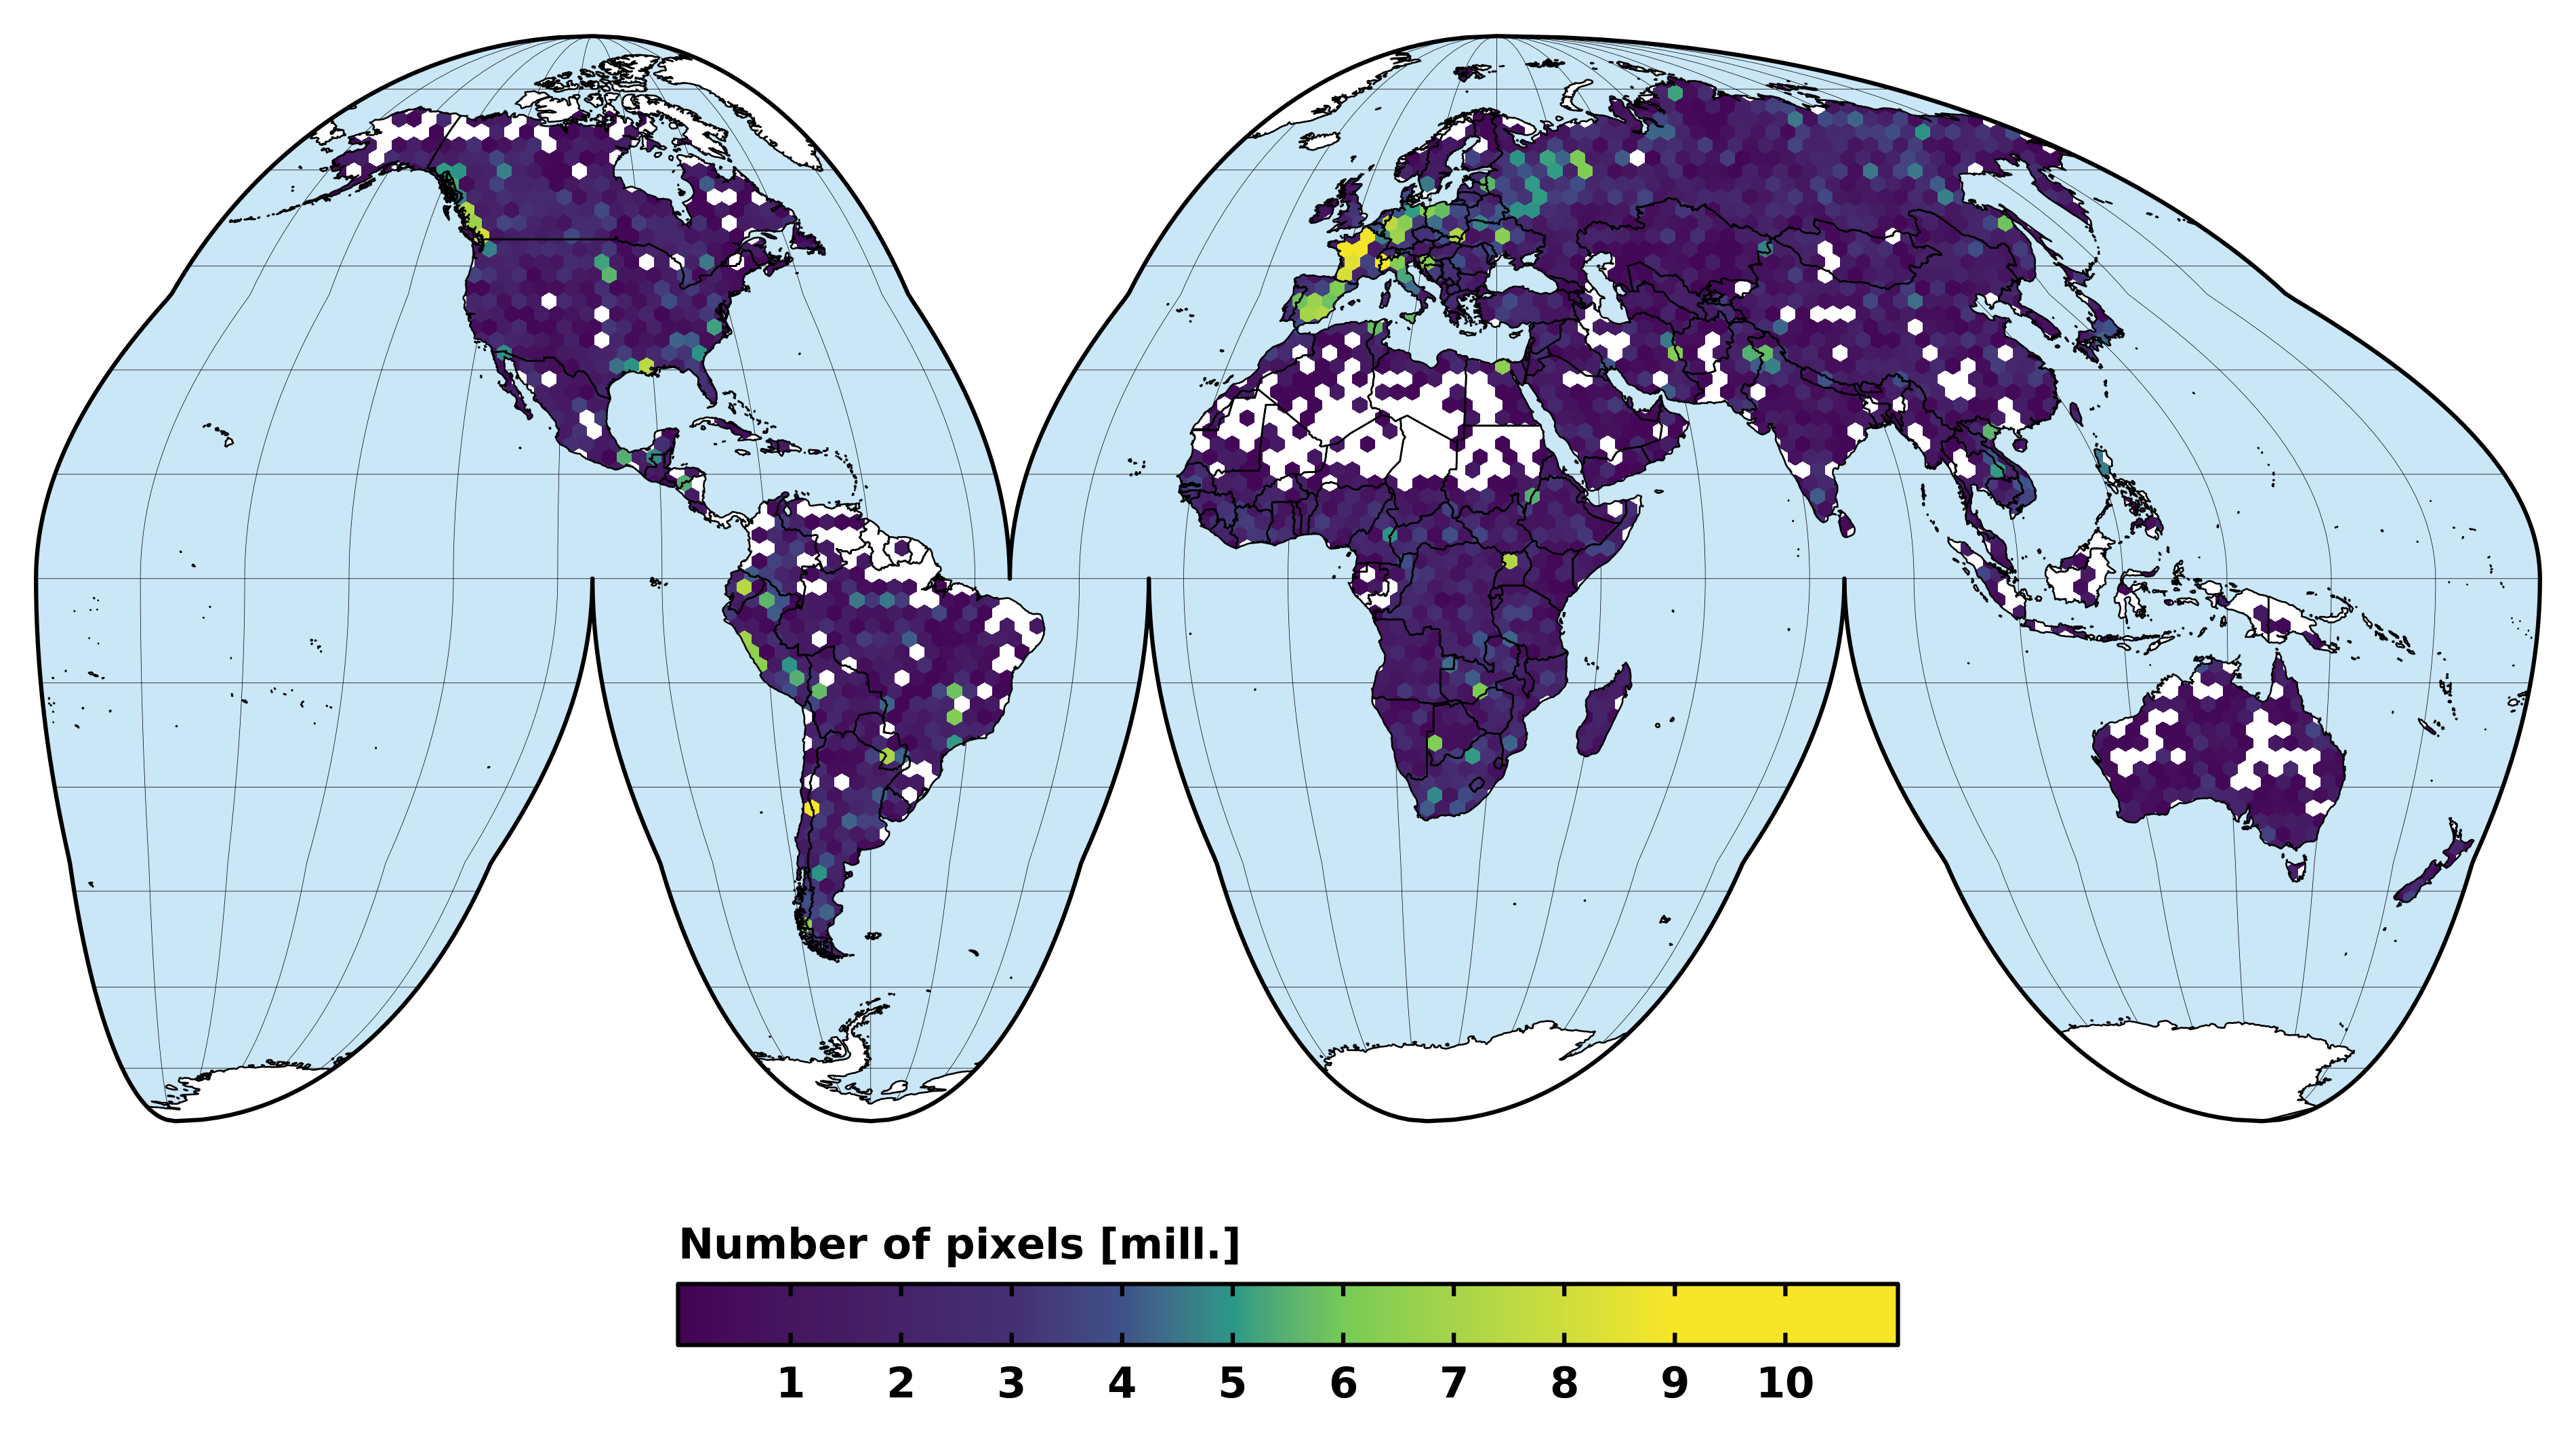
\includegraphics[width=0.98\linewidth]{figures/chapter01/figure01.png}
    \caption{CloudSEN12 spatial coverage, purple-to-yellow color gradient represents the amount of hand-crafted annotated pixels. In total in cloudSEN12 there are image patches from 10,000 different locations with five different images for each of them.}
    \label{fig:figure01}
\end{figure}

The recent progress in DL-based cloud semantic segmentation can be attributed to the proliferation of public cloud semantic segmentation datasets such as SPARCS (\cite{Hughes2019}, S2-Hollstein \cite{Hollstein2016}, Biome 8\cite{Foga2017}), 38-cloud (\cite{Mohajerani2019}), BaetensHagolle (\cite{Baetens2019}), 95-Cloud (\cite{Mohajerani2020a}), and CloudCatalogue (\cite{francis_alistair_2020_4172871}). Nonetheless, these datasets have some well-known shortcomings, including the absence of temporal features, a lack of thin clouds or cloud shadows labels, a high degree of class imbalance, and a relatively small size joined with geographical bias (see Table \ref{tab:table01} for the current characteristics/limitations of each of those datasets). Furthermore, their quality control process is not always properly described and their development remains unclear. These flaws hinder the natural transition to global DL cloud classifiers and the application of new-fashioned strategies such as few-shot learning, where model parameters can be adapted across geographies (\cite{russwurm2020meta}).

\begin{table}[!h]
    \centering
    \caption{Summary of publicly available CD datasets in comparison to CloudSEN12. An asterisk represents that the dataset does not distinguish the specific class.}
    \label{tab:table01}
    \resizebox{\textwidth}{!}{%
        \begin{tabular}{|l|c|c|c|c|c|c|c|c|c|}
            \hline
            \multicolumn{1}{|c|}{\textbf{Name}} & \textbf{Main region} & \textbf{Labels} & \textbf{\# of Scenes} & \textbf{Temporal} & \textbf{\begin{tabular}[c]{@{}c@{}}\# of Pixels\\ (10$^{9}$)\end{tabular}} & \textbf{\begin{tabular}[c]{@{}c@{}}Thick\\ Clouds \%\end{tabular}} & \textbf{\begin{tabular}[c]{@{}c@{}}Thin\\ Clouds \%\end{tabular}} & \textbf{\begin{tabular}[c]{@{}c@{}}Cloud\\ Shadows \%\end{tabular}} & \textbf{Clear \%}\\ \hline
            L8-SPARCS & worldwide & full-scene & 80 & No & 0.080 & 19.37 & * & 7.37 & 73.26\\ \hline
            S2-Hollstein & Europe & polygons & 59 & No & 0.003 & 16.06 & 16.49 & 4.53 & 62.92\\ \hline
            L8-Biome8 & worldwide & full-scene & 96 & No & 3.964 & 33.19 & 14.71 & 1.55 & 50.55\\ \hline
            L8-38Cloud & USA & full-scene & 38 & No & 1.494 & 52.36 & * & * & 47.64\\ \hline
            S2-BaetensHagolle & Europe & full-scene & 38 & No & 0.109 & 22.77$^{+}$ & * & 2.71 & 74.52\\ \hline
            L8-95Cloud & USA & full-scene & 95 & No & 3.737 & 49.27 & * & * & 50.73\\ \hline
            S2-cloudCatalog & worldwide & partial scene & 513 & No & 0.535 & 52.58 & * & 1.47 & 45.95\\ \hline
            \textbf{CloudSEN12} & \textbf{worldwide} & \textbf{partial scene} & \textbf{46697} & \textbf{Yes} & \textbf{4.5} & \textbf{xxx} & \textbf{xxx} & \textbf{xxx} & \textbf{xxx}\\ \hline
        \end{tabular}%
    }
    \footnotesize{+ Low and high cloud classes were aggregated.}
\end{table}

Inspired by the CityScapes dataset (\cite{Cordts2016}), we created and release CloudSEN12, a large and globally distributed dataset (Figure \ref{fig:figure01}) for cloud semantic understanding. CloudSEN12 surpasses all previous efforts in size and variability (Figure \ref{fig:figure02}) offering 49,250 image patches (IPs) with different annotation types: (i) 10,000 IPs with high-quality pixel-level annotation, (ii) 10,000 IPs with scribble annotation, and (iii) 29,250 unlabeled IPs. The labeling phase was conducted by 14 domain experts using a supervised active learning system. To guarantee high quality in manual annotation, we designed a rigorous four-step quality control protocol based on \cite{Zhu2019}. Furthermore, CloudSEN12 ensures that for the same geographical location, users can obtain multiple IPs with different cloud coverage: cloud-free (0\%), almost-clear (0-25\%), low-cloudy (25-45\%), mid-cloudy (45-65\%), and cloudy (\textgreater65\%), which ensures scene variability in the temporal domain.
Finally, in order to support multi-modal cloud removal\cite{Meraner2020} and data fusion\cite{Singh2018} approaches, each CloudSEN12 IP includes data from a variety of remote sensing sources that have already shown their usefulness in cloud and cloud shadow masking. See Table \ref{tab:table02} for a full list of assets available for each image patch.

\begin{table}[!h]
\centering
\caption{List of assets available for each image patch.}
\label{tab:table02}
\resizebox{\textwidth}{!}{%
  \begin{tabular}{|l|l|l|l|l|}
  \hline
  \multicolumn{1}{|l|}{\textbf{File / Folder}} & \textbf{Name} & \textbf{Scale} & \textbf{Wavelength} & \textbf{Description} \\ \hline
  \begin{tabular}[l]{@{}l@{}}S2L1C \& \\ S2L2A\end{tabular} & B1 & 0.0001 & 443.9nm (S2A) / 442.3nm (S2B) & Aerosols. \\ \cline{2-5} 
  & B2 & 0.0001 & 496.6nm (S2A) / 492.1nm (S2B) & Blue. \\ \cline{2-5} 
  & B3 & 0.0001 & 560nm (S2A) / 559nm (S2B) & Green. \\ \cline{2-5} 
  & B4 & 0.0001 & 664.5nm (S2A) / 665nm (S2B) & Red. \\ \cline{2-5} 
  & B5 & 0.0001 & 703.9nm (S2A) / 703.8nm (S2B) & Red Edge 1. \\ \cline{2-5} 
  & B6 & 0.0001 & 740.2nm (S2A) / 739.1nm (S2B) & Red Edge 2. \\ \cline{2-5} 
  & B7 & 0.0001 & 782.5nm (S2A) / 779.7nm (S2B) & Red Edge 3. \\ \cline{2-5} 
  & B8 & 0.0001 & 835.1nm (S2A) / 833nm (S2B) & NIR. \\ \cline{2-5} 
  & B8A & 0.0001 & 864.8nm (S2A) / 864nm (S2B) & Red Edge 4. \\ \cline{2-5} 
  & B9 & 0.0001 & 945nm (S2A) / 943.2nm (S2B) & Water vapor. \\ \cline{2-5} 
  & B11 & 0.0001 & 1613.7nm (S2A) / 1610.4nm (S2B) & SWIR 1. \\ \cline{2-5} 
  & B12 & 0.0001 & 2202.4nm (S2A) / 2185.7nm (S2B) & SWIR 2. \\ \hline
  S2L1C & B10 & 0.0001 & 1373.5nm (S2A) / 1376.9nm (S2B) & Cirrus. \\ \hline
  S2L2A & AOT & 0.001 & - & Aerosol Optical Thickness. \\ \cline{2-5} 
  & WVP & 0.001 & - & Water Vapor Pressure. \\ \cline{2-5} 
  & TCI\_R & 1 & - & True Color Image, Red. \\ \cline{2-5} 
  & TCI\_G & 1 & - & True Color Image, Green. \\ \cline{2-5} 
  & TCI\_B & 1 & - & True Color Image, Blue. \\ \hline
  S1 & VV & 1 & 5.405GHz & \begin{tabular}[c]{@{}l@{}}Dual-band cross-polarization,\\ vertical transmit/horizontal receive.\end{tabular} \\ \cline{2-5} 
  & VH & 1 & 5.405GHz & \begin{tabular}[c]{@{}l@{}}Single co-polarization, vertical\\ transmit/vertical receive.\end{tabular} \\ \cline{2-5} 
  & angle & 1 & - & \begin{tabular}[c]{@{}l@{}}Incidence angle generated by interpolating \\ the ‘incidenceAngle’ property.\end{tabular} \\ \hline
  \textbf{extra/} & CDI & 0.0001 & - & Cloud Displacement Index. \\ \cline{2-5} 
  & Shwdirection & 0.01 & - & \begin{tabular}[c]{@{}l@{}}Direction of cloud shadows. Values range \\ from 0°- 360°.\end{tabular} \\ \cline{2-5} 
  & elevation & 1 & - & \begin{tabular}[c]{@{}l@{}}Elevation in meters. Obtained from \\ MERIT Hydro datasets.\end{tabular} \\ \cline{2-5} 
  & ocurrence & 1 & - & \begin{tabular}[c]{@{}l@{}}JRC Global Surface Water. The frequency \\ with which water was present.\end{tabular} \\ \cline{2-5} 
  & LC100 & 1 & - & \begin{tabular}[c]{@{}l@{}}Copernicus land cover product.\\ CGLS-LC100 Collection 3.\end{tabular} \\ \cline{2-5} 
  & LC10 & 1 & - & \begin{tabular}[c]{@{}l@{}}ESA WorldCover 10m v100 \\ product.\end{tabular} \\ \hline
  \multicolumn{1}{|l|}{\textbf{labels/}} & fmask & 1 & - & Fmask4.0 cloud masking. \\ \cline{2-5} 
  \multicolumn{1}{|l|}{} & QA60 & 1 & - & SEN2 Level-1C cloud mask. \\ \cline{2-5} 
  \multicolumn{1}{|l|}{} & s2cloudless & 1 & - & sen2cloudless results. \\ \cline{2-5} 
  \multicolumn{1}{|l|}{} & sen2cor & 1 & - & \begin{tabular}[c]{@{}l@{}}Scene Classification band. Obtained from \\ SEN2 level 2A.\end{tabular} \\ \cline{2-5} 
  \multicolumn{1}{|l|}{} & DL\_L8S2\_UV\_rgbi & 1 & - & \begin{tabular}[c]{@{}l@{}} \cite{Lopez-Puigdollers2021} results \\ based on RGBI bands.\end{tabular} \\ \cline{2-5} 
  \multicolumn{1}{|l|}{} & DL\_L8S2\_UV\_rbgiswir & 1 & - & \begin{tabular}[c]{@{}l@{}} \cite{Lopez-Puigdollers2021} results \\ based on RGBISWIR bands.\end{tabular} \\ \cline{2-5}
  \multicolumn{1}{|l|}{} & kappamask\_L1C & 1 & - & \begin{tabular}[c]{@{}l@{}} KappaMask results using SEN2 \\ level L1C as input.\end{tabular} \\ \cline{2-5}
  \multicolumn{1}{|l|}{} & kappamask\_L2A & 1 & - & \begin{tabular}[c]{@{}l@{}} KappaMask results using SEN2 \\ level L2A as input.\end{tabular} \\ \cline{2-5}         
  & manual\_hq & 1 &  & \begin{tabular}[c]{@{}l@{}}High-quality pixel-wise manual annotation.\end{tabular} \\ \cline{2-5} 
  & manual\_sc & 1 &  & \begin{tabular}[c]{@{}l@{}}Scribble manual annotation. \end{tabular} \\ \hline
  \end{tabular}
}
\end{table}

\hypertarget{methods}{%
\section{Methods}\label{methods}}

This study starts by collecting and combining several public data sources that potentially may help us better comprehend cloud and cloud shadow semantics. Based on this information, semantic classes (Table\textasciitilde{}\ref{tab:table03}) are created using an active system that blends human photo-interpretation and machine learning. Finally, a strict quality control protocol is carried out to ensure the highest quality on the manual labels and to standardize human-level performance. Figure \ref{fig:figure03} depicts the workflow followed to create the dataset.

\begin{figure}[!h]
    \centering
    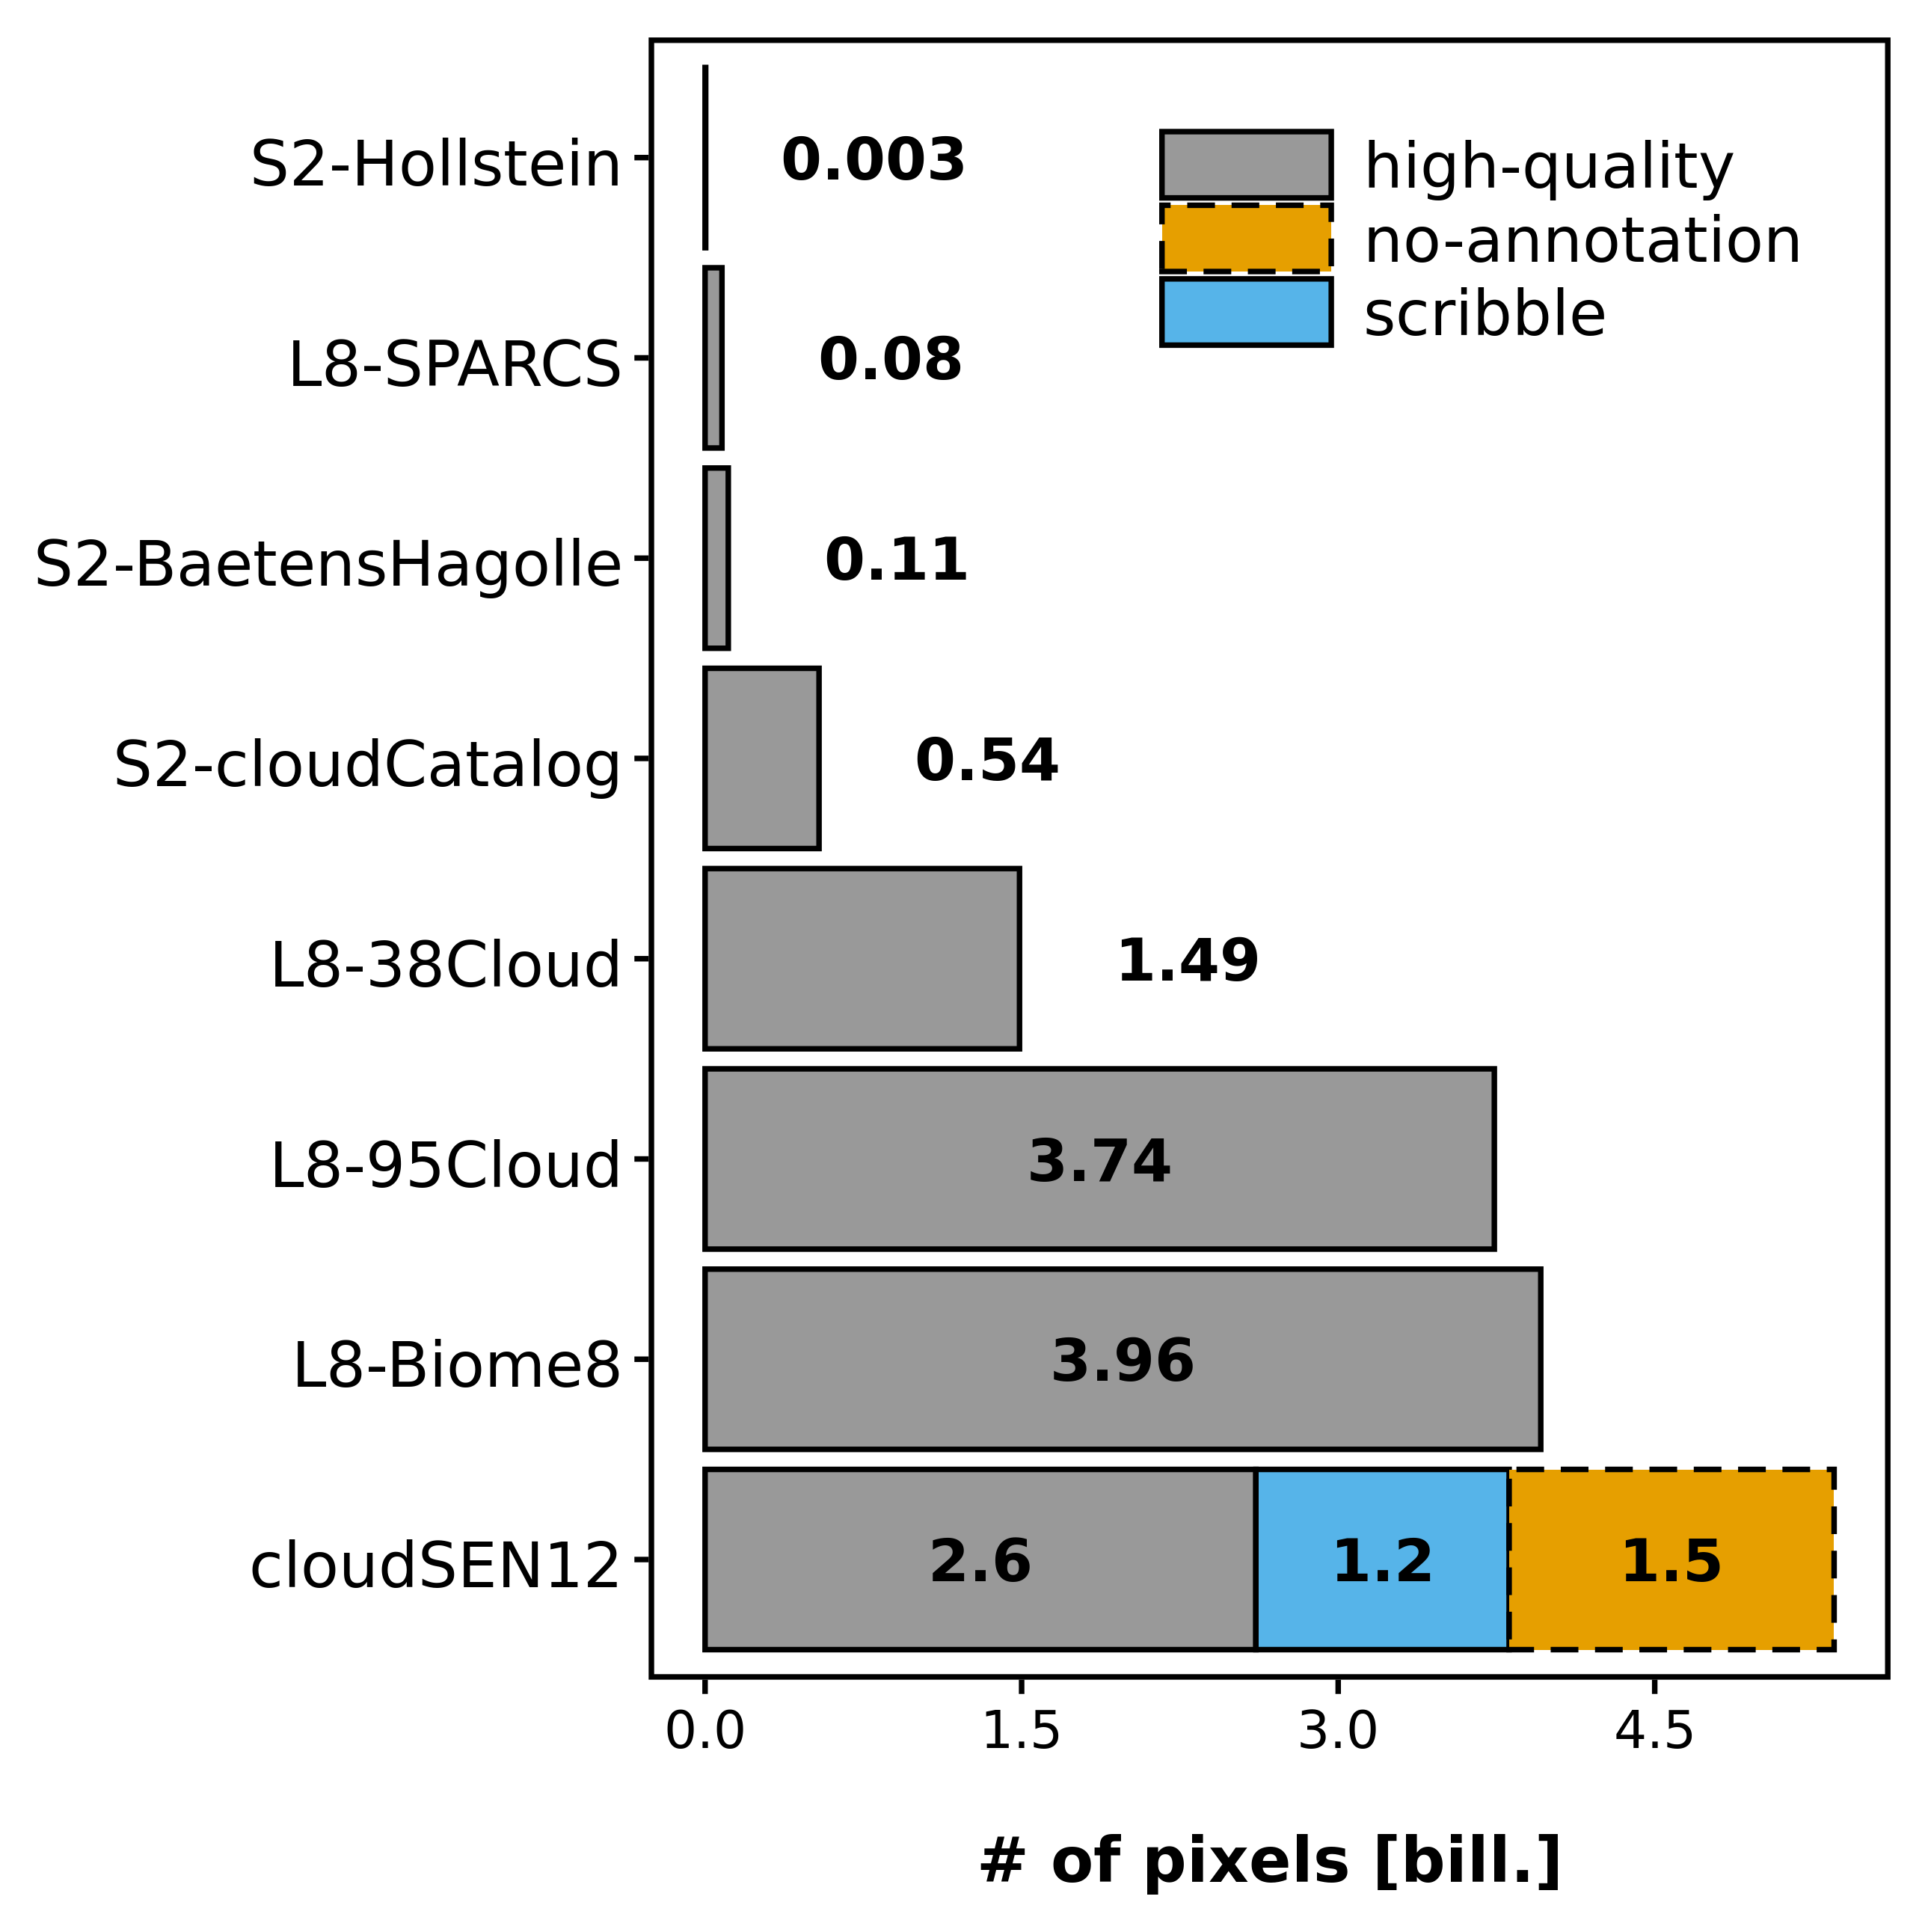
\includegraphics[width=0.7\linewidth]{figures/chapter01/figure02.png}
    \caption{Number of hand-crafted pixel annotations between different cloud detection datasets. All the labeled pixels in the CloudSEN12 no-annotation group come from cloud-free IPs.}
    \label{fig:figure02}
\end{figure}

\begin{figure}[!h]
    \centering
    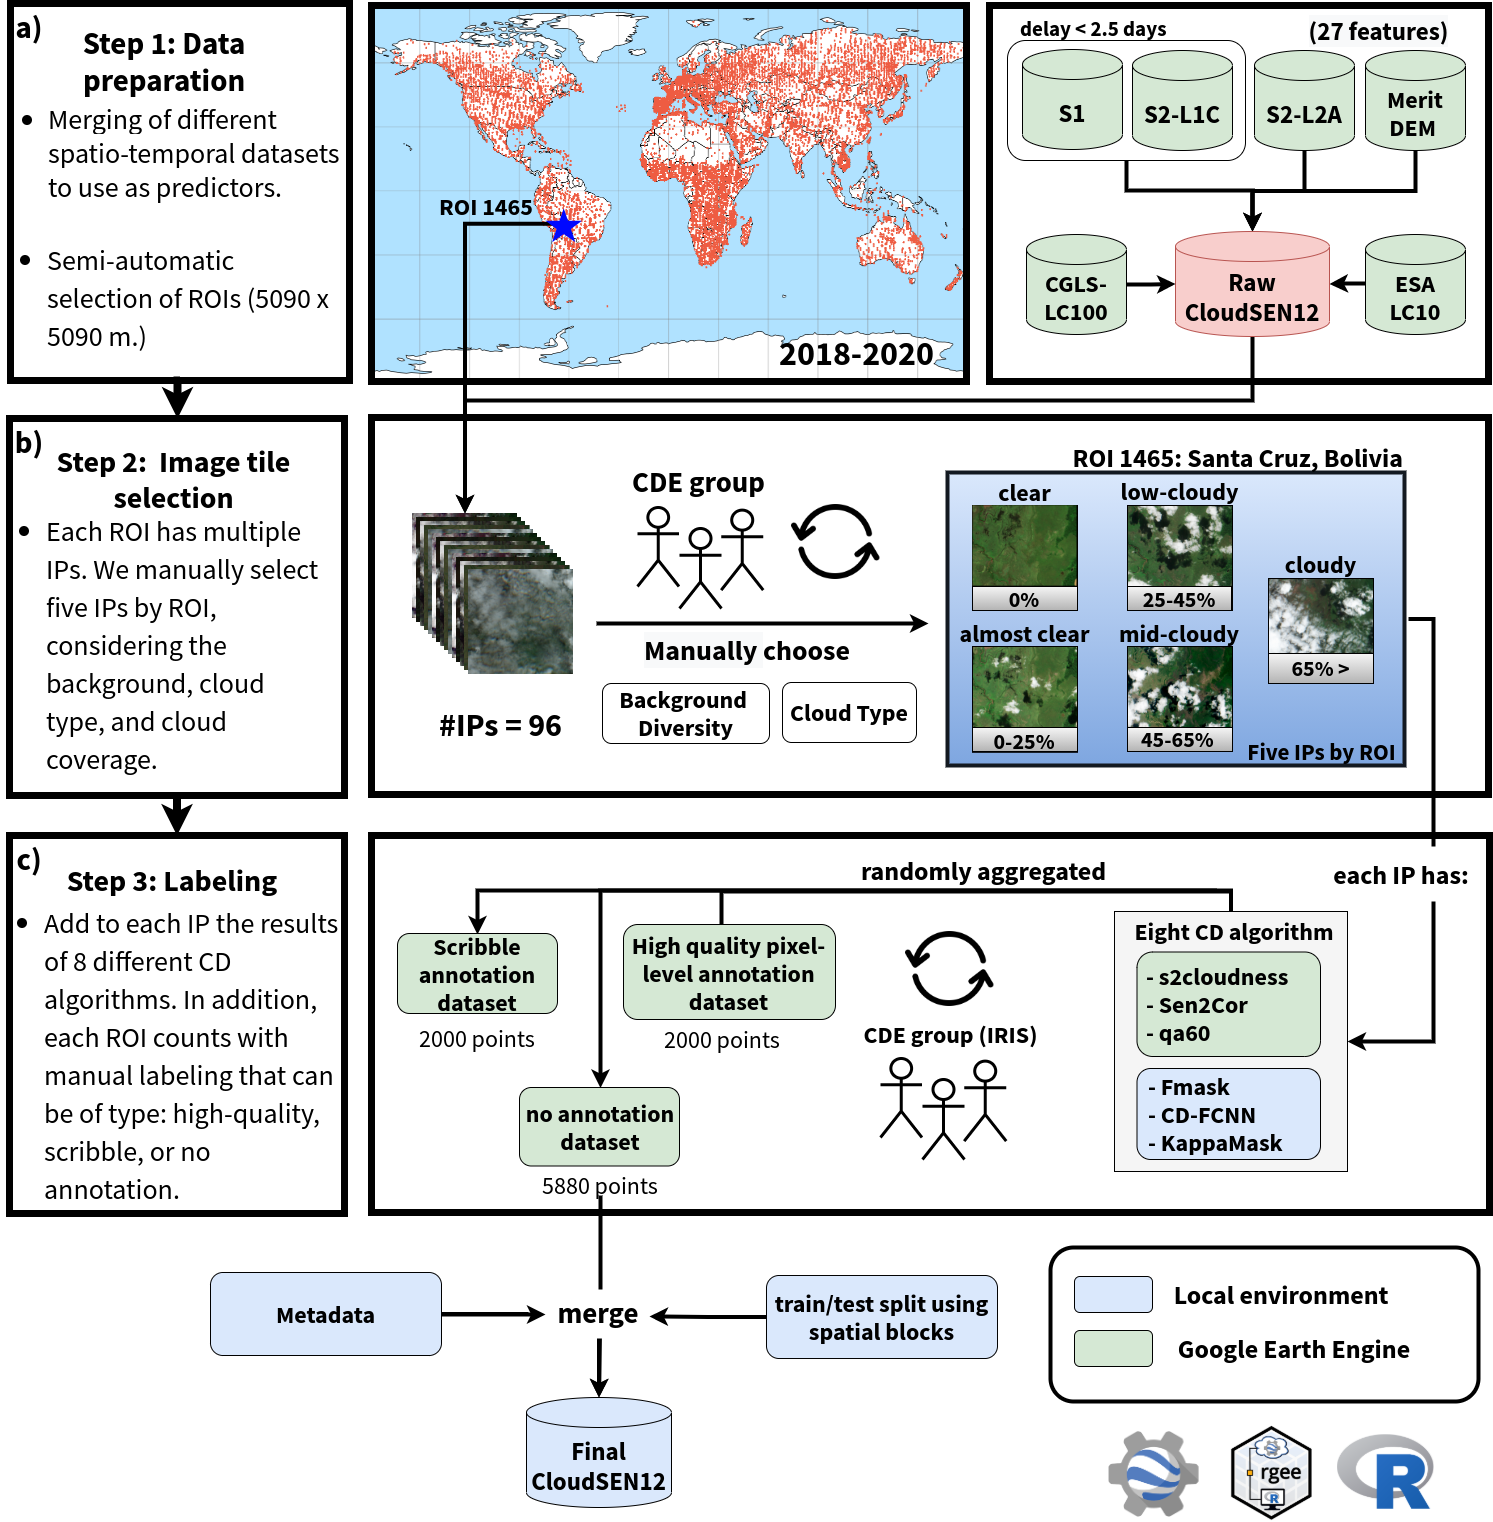
\includegraphics[width=0.98\linewidth]{figures/chapter01/figure03.png}
    \caption{A high-level summary of our workflow to generate IPs. a) Satellite imagery datasets that comprises CloudSEN12 assets. b) IP selection by the CDE group. c) Generation of manual and automatic cloud masking.}
    \label{fig:figure03}
\end{figure}

\hypertarget{data-preparation}{%
\subsection{Data preparation}\label{data-preparation}}

CloudSEN12 comprises different free and open datasets provided by several public institutions and made accessible by the Google Earth Engine (GEE) platform\cite{Gorelick2017}. These include Sentinel-2A/B (SEN2), Sentinel-1 (SEN1), Multi-Error-Removed Improved-Terrain (MERIT) DEM\cite{Yamazaki2019}, Global Surface Water\cite{Pekel2016} (GSW), and Global Land Cover maps\cite{Buchhorn2020} at 10 and 100 meters. The SEN2 multi-spectral image data corresponds to the 2018--2020 period. We included all the bands from both SEN2 top-of-atmosphere (TOA) reflectance (Level-1C) and SEN2 surface reflectance (SR) values (Level-2A) derived from the Sen2Cor processor, which can be useful to analyze the impact of CD algorithms on atmospherically corrected derived products. See \textit{S2L1C} and \textit{S2L2A} in Table \ref{tab:table02} for band description. Previous studies have proven the reliability of TOA\cite{Zekoll2021} and SR values for cloud detection, but SR data revealed a more plausible differentiation between cloud shadows and clear pixels\cite{Domnich2021}. On the other hand, SEN1 acquires data with a revisit cycle between 6-12 days according to four standard operational modes: Stripmap (SM), Extra Wide Swath (EW), Wave (WV), and Interferometric Wide Swath (IW). In CloudSEN12, we collect IW data with two polarization channels (VV and VH) from the high-resolution Level-1 Ground Range Detected (GRD) product. Furthermore, we saved the approximate angle between the incident SAR beam and the reference ellipsoid (see \textit{S1} in Table \ref{tab:table02}). Lastly, our dataset also includes previously proposed features for cloud semantic segmentation such as (1) Cloud Displacement Index\cite{Frantz2018}, (2) the direction of cloud shadow (0 - 360°) calculated using the solar azimuth and zenith angles\cite{FernandezMoranPHOTO21} from SEN2 metadata, (3) elevation from MERIT dataset, (4) land cover maps from the Copernicus Global Land Service (CGLS) version 3, and the ESA WorldCover 10m v100, and (5) water occurrence from the GSW dataset (see \textit{extra/} in Table \ref{tab:table02}). All the previous features constitute the raw CloudSEN12 imagery dataset (Figure \ref{fig:figure03}a). In raw CloudSEN12, full image scenes were resampled to 10 meters using local SEN2 UTM coordinates.

\begin{table}[!h]
    \centering
    \caption{Cloud semantic categories considered CloudSEN12}
    \label{tab:table03}
    \resizebox{\textwidth}{!}{%
    \begin{tabular}{|l|l|l|l|l|}
        \hline
        \textbf{Code} & \textbf{Class} & \textbf{Superclass} & \textbf{Description} & \textbf{Priority} \\ \hline
        0 & Clear  & Valid & Pixels without cloud and cloud shadow contamination. & 4 \\ \hline
        1 & Thick Cloud  & Invalid  & \begin{tabular}[c]{@{}l@{}} Opaque clouds that block all the reflectance from \\ the Earth’s surface.\end{tabular} & 1 \\ \hline
        2 & Thin Cloud  & Invalid  & \begin{tabular}[c]{@{}l@{}} Semitransparent cloud that modifies the background\\ signal.\end{tabular} & 3 \\ \hline
        3 & Cloud Shadow  & Invalid  & Dark pixels thrown by a thick or thin cloud. & 2 \\ \hline
    \end{tabular}
    }
\end{table}

\hypertarget{image-patches-selection}{%
\subsection{Image patches selection}\label{image-patches-selection}}

In order to gather the raw CloudSEN12 data, we sampled 20,000 random regions of interest (ROIs) distributed worldwide. Each ROI has a dimension of 5,090x5,090 square meters. Besides, we carefully added 5,000 manual selected ROIs to guarantee high scene diversity on complicated surfaces such as snow and built-up areas. After that, a ROI is retained in the dataset if all three of the following requirements are met: (1) SEN2 Level-1C IP does not include saturated, defective, or no-data pixel values, (2) the time difference between SEN1 and SEN2 acquisitions is not higher than 2.5 days, and (3) there are more than 15 SEN2 Level-1C image scenes for the given ROI after applying (2). The total number of ROIs decreased from 25,000 to 12,121 as a result of this filtering. Despite this reduction, CloudSEN12 still manages to reach a full global representation (see Figure \ref{fig:figure01}). However, a high number of ROIs does not necessarily imply a consistent distribution among cloud types and cover. Unfortunately, automated image selection based on automatic cloud masking or cloud cover metadata tends to produce misleading results, especially under high-altitude areas\cite{dirk2021}, intricate backgrounds \cite{Rittger2020}, and mixed cloud types scenes. Hence, to guarantee unbiased distribution between clear, cloud and cloud shadow pixels, 14 cloud detection experts manually selected IPs (hereafter referred to as CDE group, Figure \ref{fig:figure03}b). For each ROI, we pick five IPs with different cloud coverage: cloud-free (0\%), almost-clear (0-25\%), low-cloudy (25-65\%), mid-cloudy (45-65\%), and cloudy image (\textgreater65\%). Atypical clouds such as contrails, ice clouds, and haze/fog had a higher priority than common clouds (i.e., cumulus and stratus). After eliminating ROIs that did not count with at least one IP for each cloud coverage class, the total number of ROIs was reduced from 12,121 to 9,880, resulting in the final CloudSEN12 spatial coverage (Figure \ref{fig:figure01}).

\begin{figure}[!h]
    \centering
    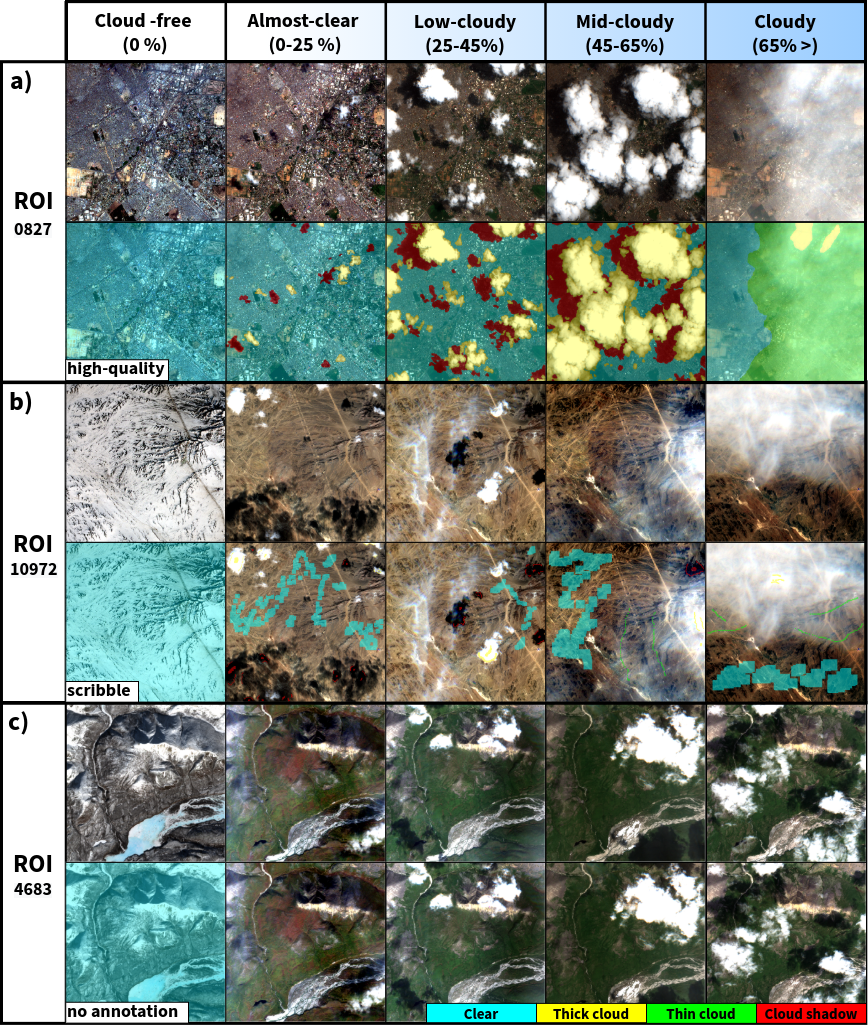
\includegraphics[width=0.98\linewidth]{figures/chapter01/figure04.png}
    \caption{The three primary forms of hand-crafted labeling data in CloudSEN12. a) high-quality, the rows depict: SEN2 level 1C data in RGB, manual\_hq (high-quality), manual\_sc (high-quality).}
    \label{fig:figure04}
\end{figure}

\hypertarget{annotation-strategy}{%
\subsection{Annotation strategy}\label{annotation-strategy}}

New trends in computer vision shows that reformulating the standard supervised learning scheme can alleviate the huge demands of hand-crafted labeled data. Semi-supervised learning, for instance, can produce more detailed and uniform predictions in semantic segmentation \cite{Castillo-Navarro2020}. While weakly-supervised learning suggests a more cost-effective option to pixel-wise annotation, users might utilize scribble labels to train a learning signal for coarse-to-fine enrichment\cite{Li2020a}. Aware of these manual labeling requirements, CloudSEN12 also supports weakly and self-/semi-supervised learning strategies by including three distinct forms of labeling data: high-quality, scribble, and no-annotation. Consequently, each ROI is randomly assigned to a different annotation group:

\begin{itemize}
    \item 2,000 ROIs with pixel level annotation, where the average annotation time is 150 minutes (high-quality group, Figure \ref{fig:figure04}a).
    \item 2,000 ROIs with scribble level annotation, where the annotation time is 15 minutes (scribble group, Figure \ref{fig:figure04}b).
    \item 5,880 ROIs with annotation only in the cloud-free (0\%) image (no annotation group, Figure \ref{fig:figure04}c).
\end{itemize}

\begin{figure}[!h]
    \centering
    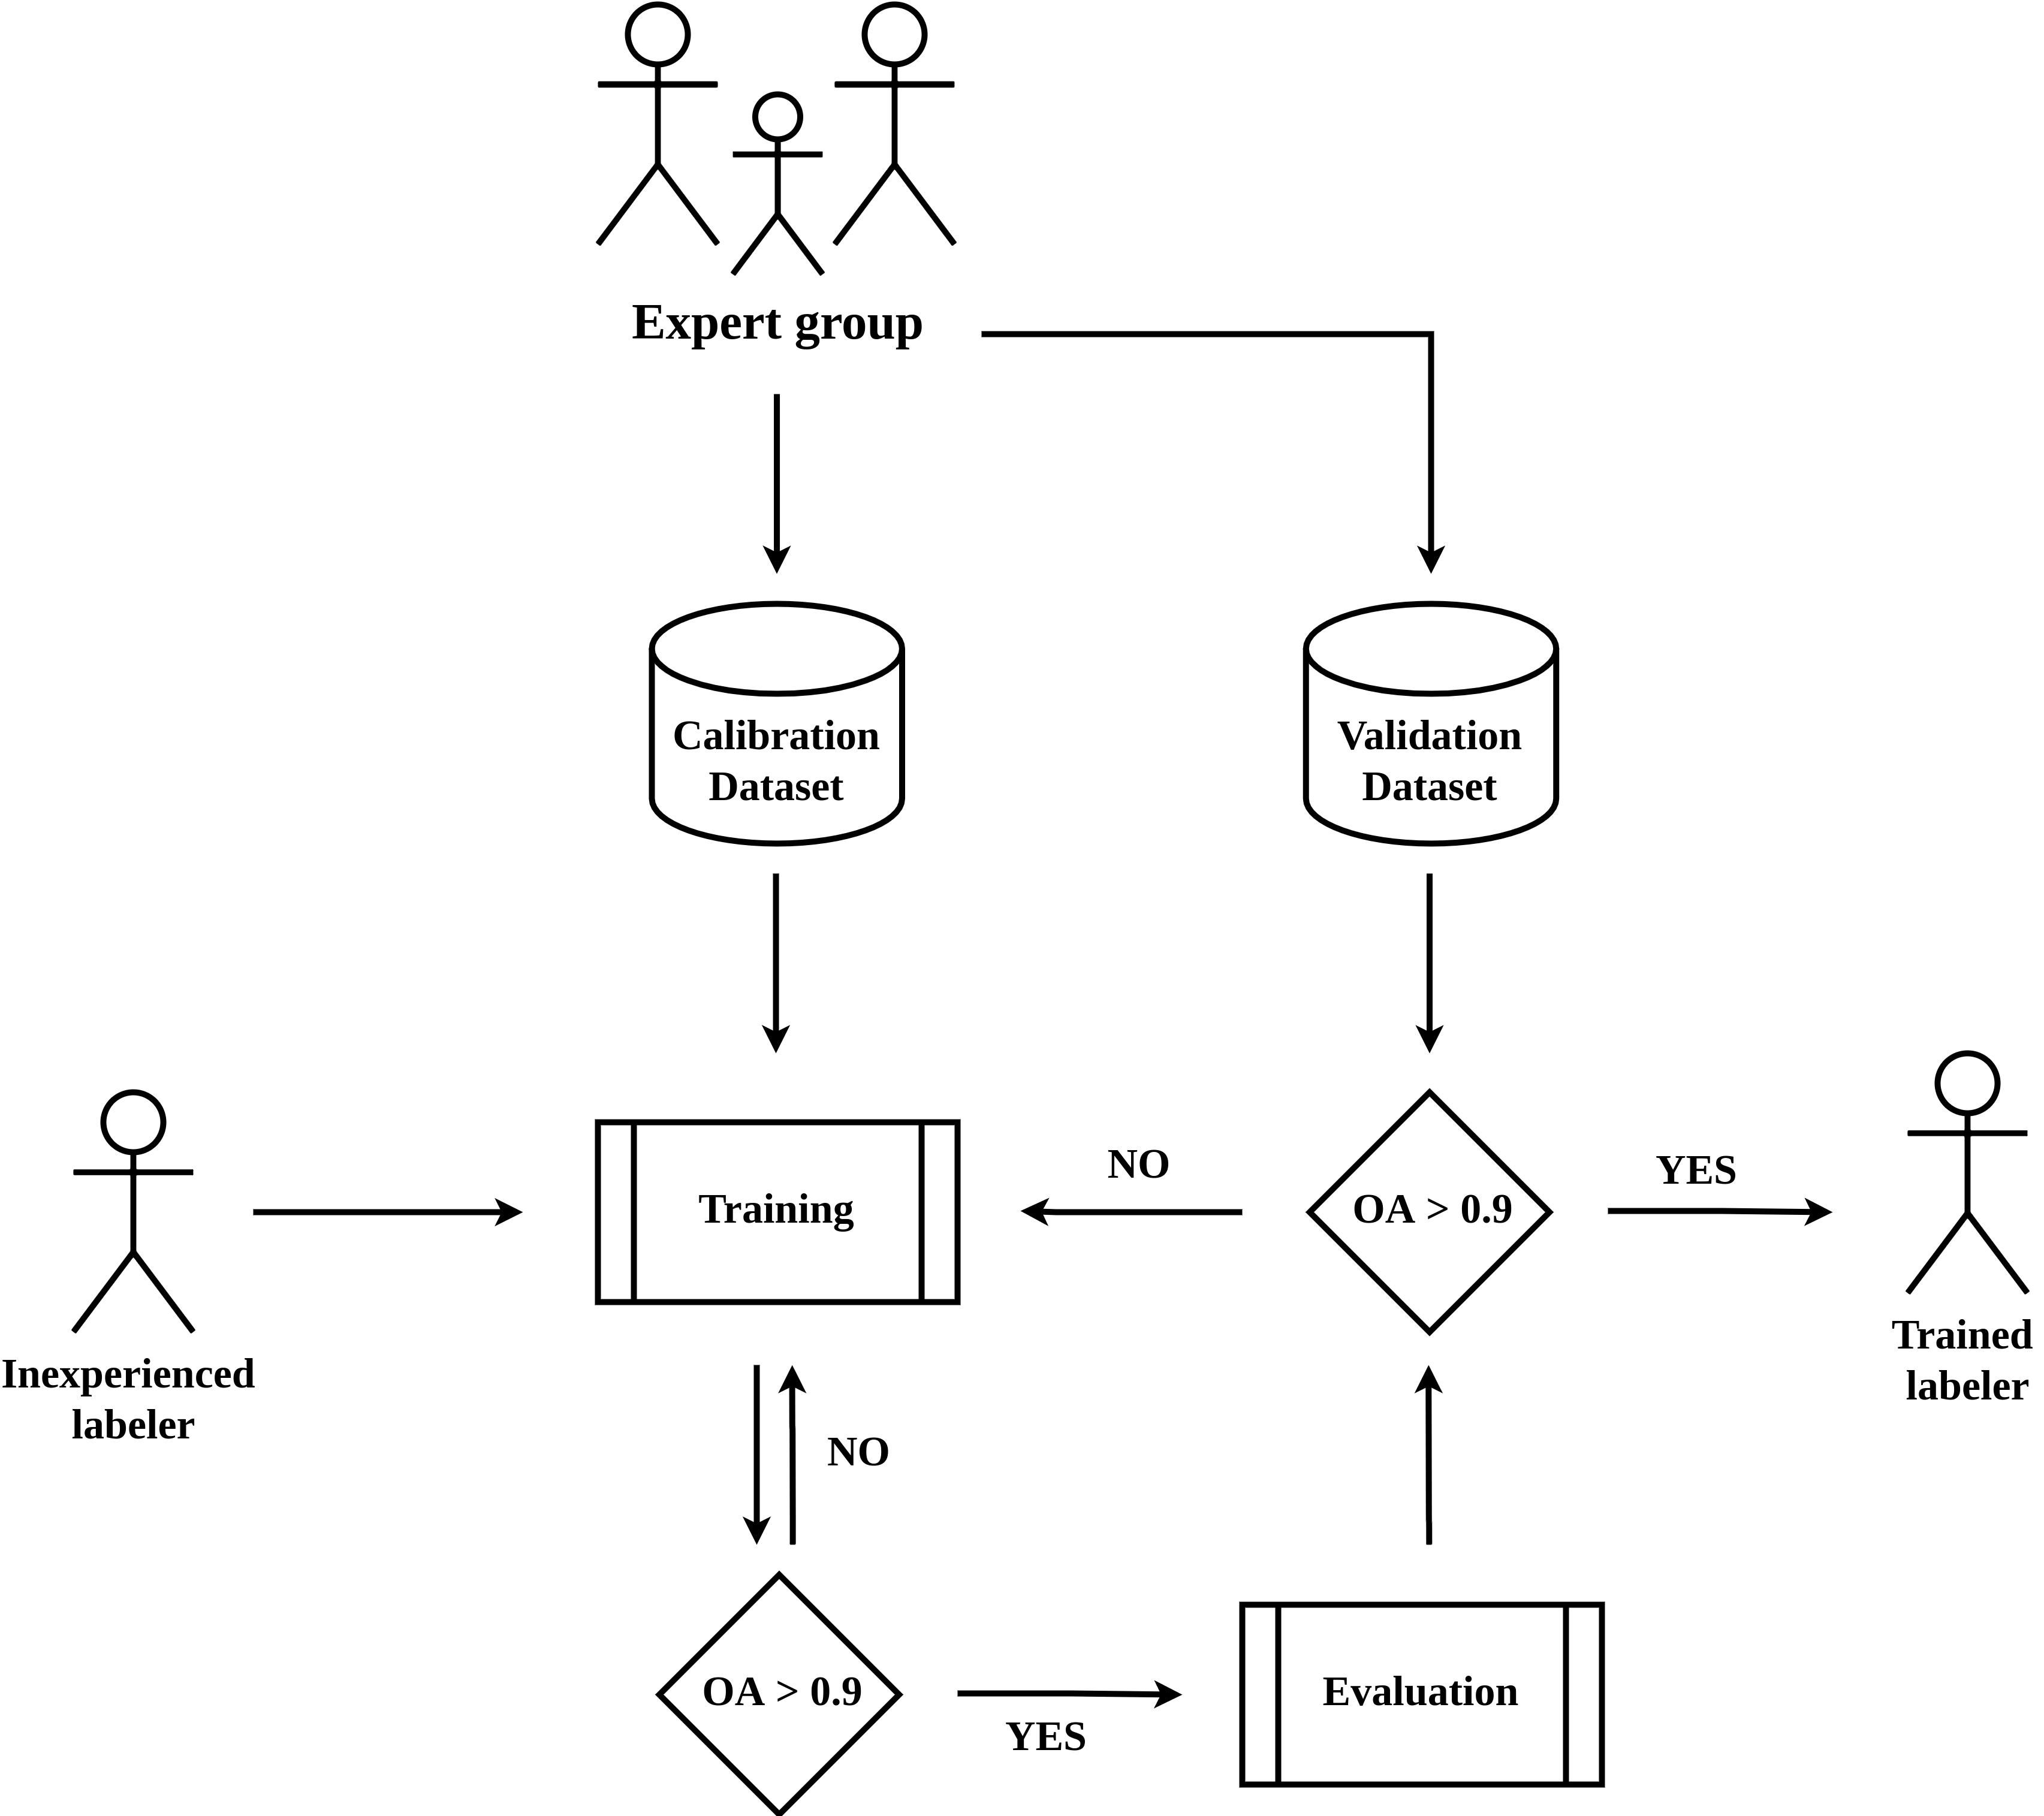
\includegraphics[width=0.98\linewidth]{figures/chapter01/figure05.png}
    \caption{Human calibration phase diagram. The overall accuracy (OA) is measured comparing the inexperienced labeler against the expert group results.}
    \label{fig:figure05}
\end{figure}

\hypertarget{human-calibration-phase}{%
\subsection{Human calibration phase}\label{human-calibration-phase}}

Human-made photo interpretation is not a faultless procedure. It might easily be skewed by an individual's basis, overconfidence, tiredness, or ostrich-effect\cite{Valdez2017} proclivity. Hence, to lessen this concern, the CDE group refined their criteria using a \texttt{calibration\textquotesingle{}\textquotesingle{}\ dataset\ composed\ of\ 35\ manually\ selected\ challenging\ IPs.\ In\ this\ stage,\ all\ the\ labelers\ can\ consult\ each\ other.\ As\ a\ result,\ they\ reached\ an\ agreement\ about\ the\ SEN2\ band\ compositions\ to\ be\ used\ and\ how\ to\ deal\ with\ complicated\ scenarios\ such\ as\ cloud\ boundaries,\ thin\ cloud\ shadows,\ and\ high-reflectance\ background.\ A\ labeler\ is\ considered\ fully\ trained\ if\ its\ overall\ accuracy\ in\ the\ calibration\ dataset\ surpasses\ 90\textbackslash{}\%.\ Then,\ a}validation'\,' dataset formed of ten IPs is used to assess individual performance; labelers are not permitted to confer with one another during this step. If the labeler's overall accuracy drops below 90\%, it will return to the calibration phase (Figure \ref{fig:figure05}). The human-level performance is measured by comparing the individual labeler's result before and after our four-step control quality procedure (see quality control section). As shown in Figure \ref{fig:figure06}, CloudSEN12 set the human-level performance at 95\% confidence, varying according to the IP difficulty metadata (see Table \ref{tab:table04}) from 98 to 85\%.

\begin{table}[!h]
    \centering
    \caption{Metadata associated to each image patch.}
    \label{tab:table04}
    \resizebox{\textwidth}{!}{%
    \begin{tabular}{|l|l|}
        \hline
        \textbf{Metadata name} & \textbf{Description} \\ \hline
        annotator\_name & The labeler's name. \\ \hline
        roi\_id & The region of interest ID. \\ \hline
        s2\_id\_gee & Sentinel-2 GEE ID. \\ \hline
        s2\_id & Sentinel-2 product ID. \\ \hline
        s2\_date & Sentinel-2 acquisition date in ISO format. \\ \hline
        s2\_sen2cor\_version & \begin{tabular}[c]{@{}l@{}}Sen2Cor configuration baseline used at the time of the product \\
        generation.\end{tabular} \\ \hline
        s2\_fmask\_version & Fmask version. \\ \hline
        s2\_s2cloudless\_version & s2cloudless version. \\ \hline
        s2\_reflectance\_conversion\_correction & Earth-Sun distance correction factor. \\ \hline
        s2\_aot\_retrieval\_accuracy & Accuracy of aerosol optical thickness model. \\ \hline
        s2\_water\_vapour\_retrieval\_accuracy & Declared accuracy of the Water Vapor model. \\ \hline
        s2\_view\_off\_nadir & \begin{tabular}[c]{@{}l@{}}The angle from the SEN2 sensor between nadir (straight down) and\\ the scene center.\end{tabular} \\ \hline
        s2\_view\_sun\_azimuth & SEN2 sun azimuth angle. \\ \hline
        s2\_view\_sun\_elevation & SEN2 sun elevation angle. \\ \hline
        s1\_id & SEN1 product ID. \\ \hline
        s1\_date & SEN1 acquisition date in ISO format. \\ \hline
        s1\_grd\_post\_processing\_software\_name & Name of the software to pre-processing SEN1. \\ \hline
        s1\_grd\_post\_processing\_software\_version & SEN1 software pre-processing version. \\ \hline
        s1\_slc\_processing\_facility\_name & Name of the facility where the processing step was performed. \\ \hline
        s1\_slc\_processing\_software\_version & Software version identification. \\ \hline
        s1\_radar\_coverage & percentage of valid SEN1 pixels contained in this IP. \\ \hline
        land\_cover & Predominant land use. \\ \hline
        label\_type & Manual labeling type (i.e., scribble, high-quality or no-annotation). \\ \hline
        cloud\_coverage & \begin{tabular}[c]{@{}l@{}} Cloud coverage estimated using photo-interpretation. \\(see section: Image patches selection).\end{tabular} \\ \hline
        test & Whether the IP is part of training (train) or testing (test) dataset. \\ \hline
        difficulty & \begin{tabular}[c]{@{}l@{}}Labeler's confidence (from 1 to 5) of the manual annotation.Where\\ one indicates near-perfect and five denotes potentially significant mistakes.\end{tabular} \\ \hline        
        proj:epsg & EPSG code. \\ \hline
        proj:geometry & Footprint of this IP. \\ \hline
        proj:shape & Number of pixels for the default IP. \\ \hline
        proj:centroid & Centroid coordinates of the IP in latitude and longitude. \\ \hline
        proj:transform & The affine transformation coefficients. \\ \hline
    \end{tabular}}
\end{table}

\begin{figure}[!h]
    \centering
    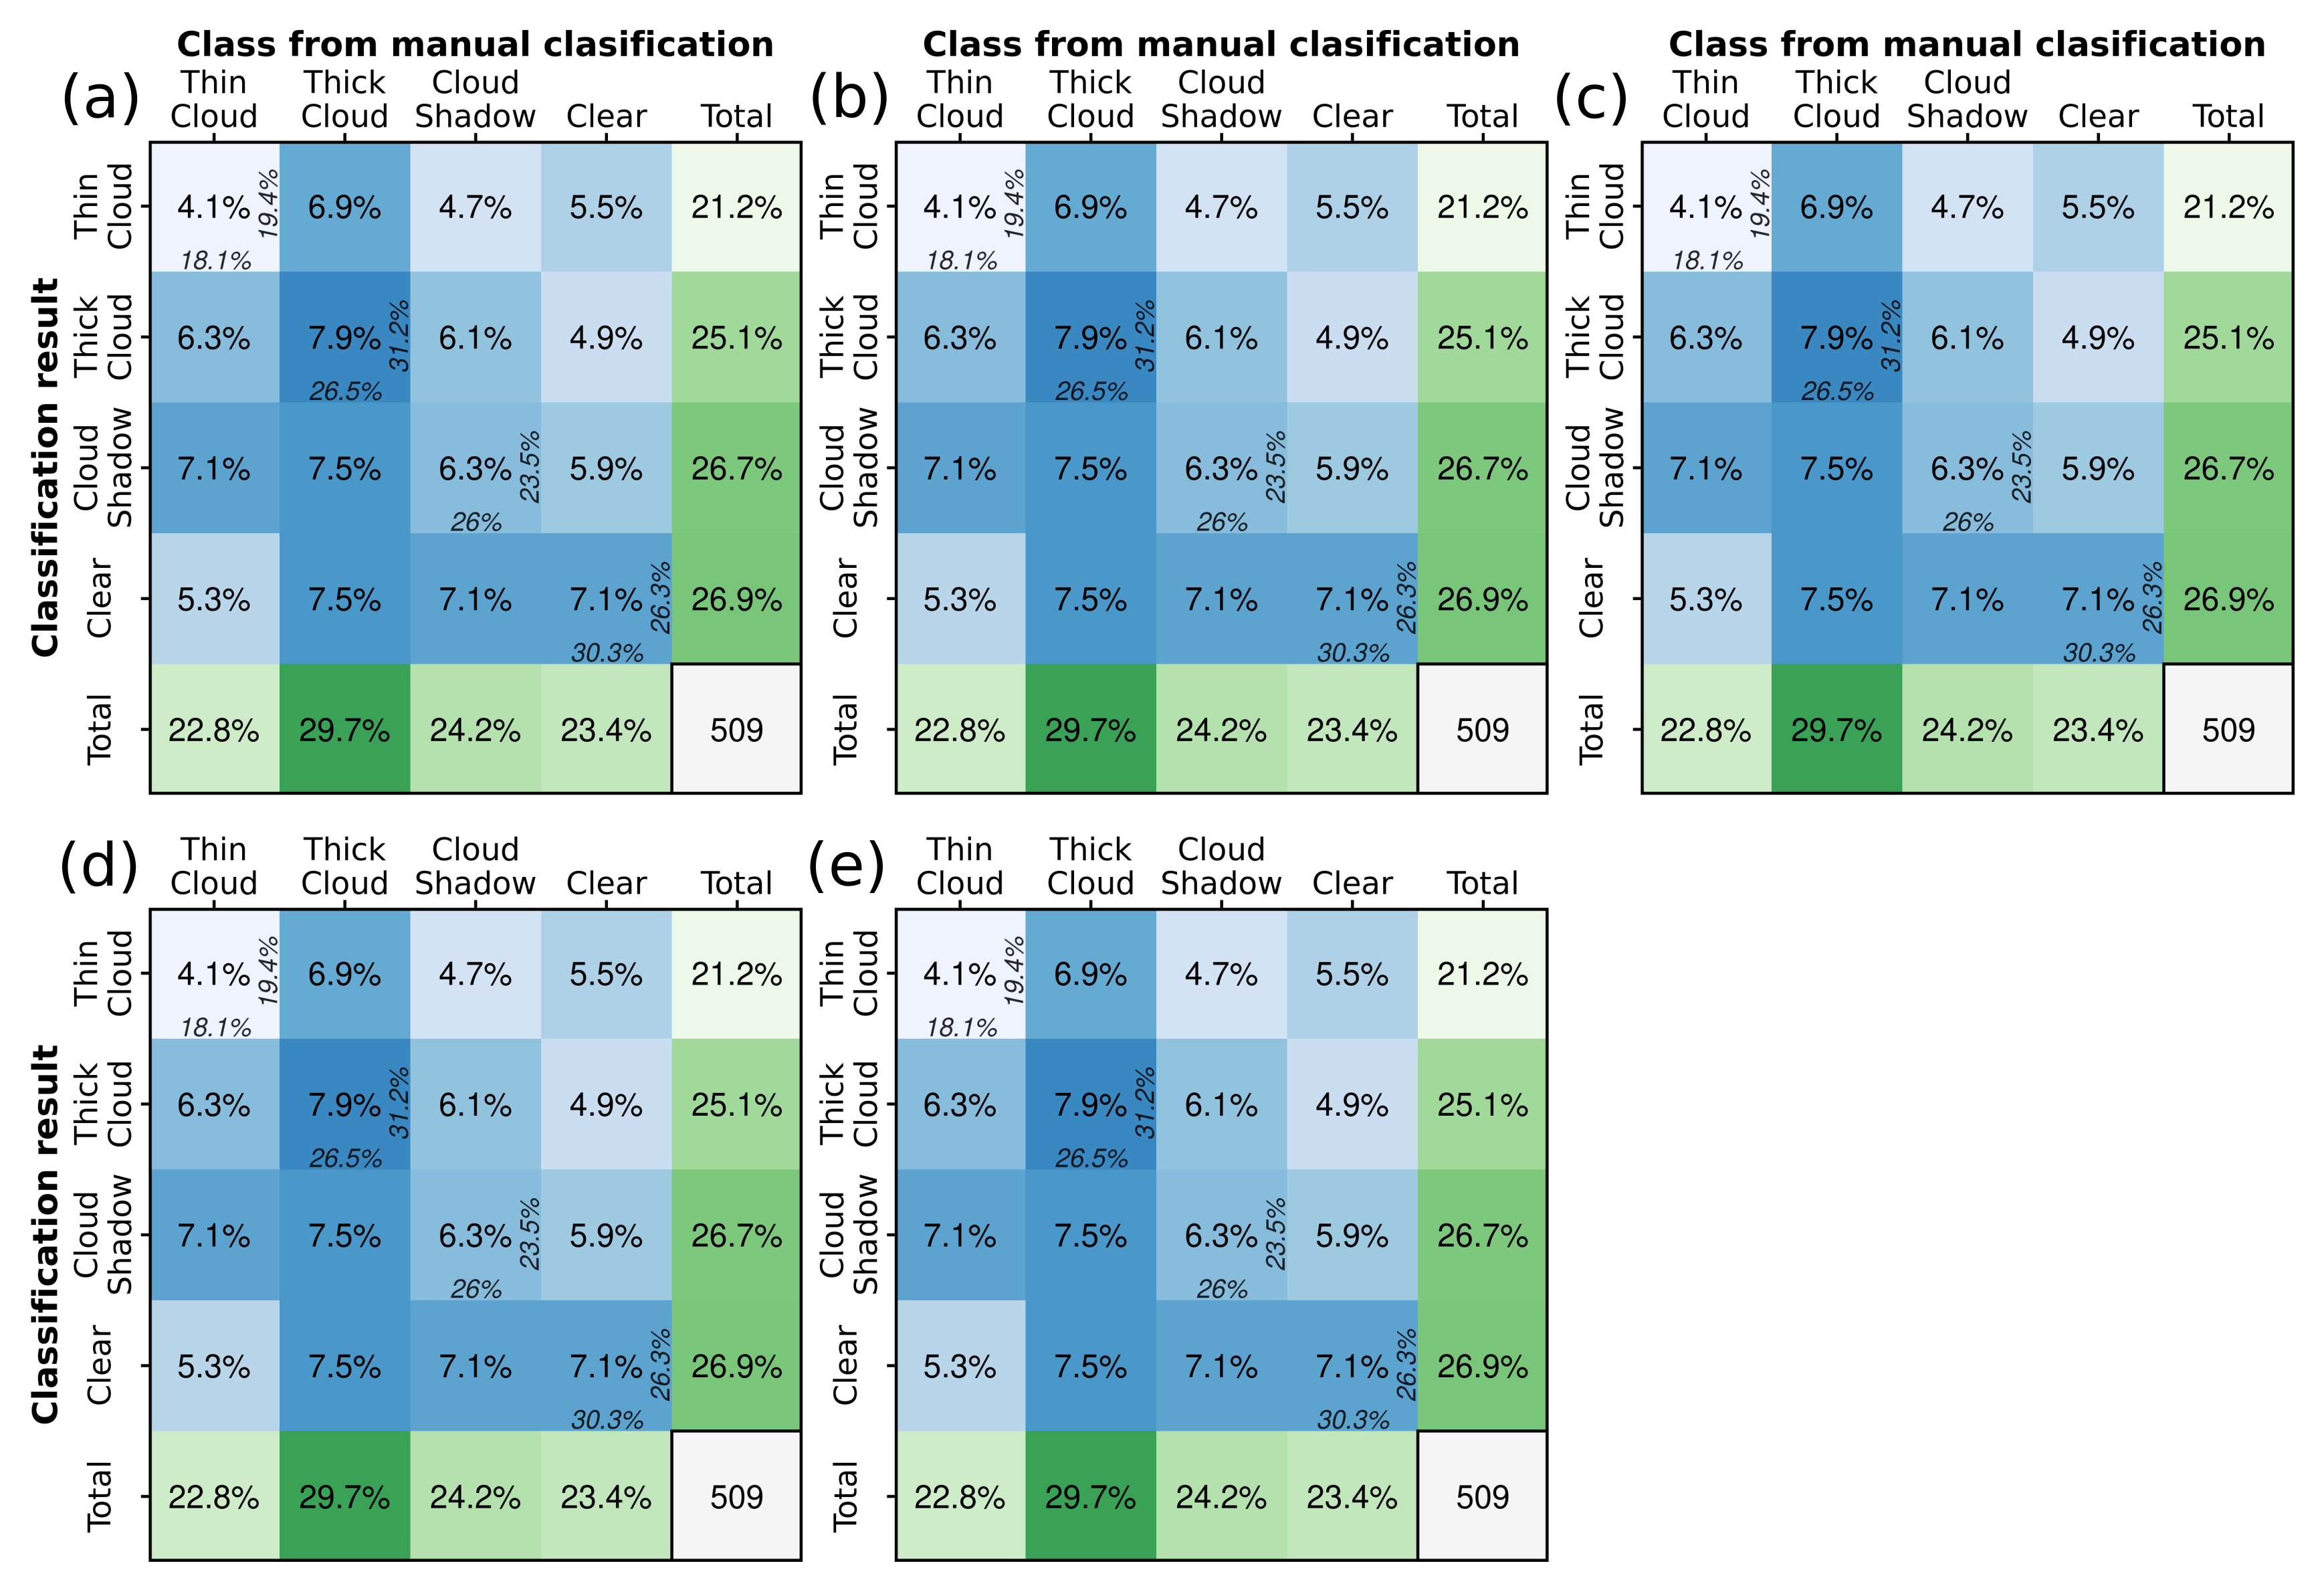
\includegraphics[width=0.98\linewidth]{figures/chapter01/figure06.png}
    \caption{Confusion matrices (values in percent) between the high-quality manual labels cast by the CDE group after and before the quality control process. See the sections human calibration and quality control. The original labels are divided based on the difficulty IP property (See Table \ref{tab:table04}).}
    \label{fig:figure06}
\end{figure}

\hypertarget{labeling-phase}{%
\subsection{Labeling phase}\label{labeling-phase}}

The Intelligence foR Image Segmentation (IRIS) active learning software\cite{iris2019} was used in the manual labeling annotation process (Supplementary Figure \ref{fig:figureS01}). IRIS allowed CDE members to train a model (learner) with a small set of labeled samples that is iteratively reinforced by acquiring new samples provided by a labeler (oracle). As a result, it dramatically decreases the time spent creating hand-crafted labels but maintaining the labeler's capacity to make final manual revisions if necessary. For high-quality labeling generation (Figure \ref{fig:figure07}a), IRIS starts training a gradient boosting decision tree (GBDT) with s2cloudless cloud probability values greater than 0.7 as thick cloud and less than 0.3 as clear. Next, the labelers make adjustments to the prior results and, if necessary, add other cloud semantic classes such as cloud shadow and thin cloud. Using this new sample set, the GBDT model is re-trained. The two previous steps are repeated several times until the pixel-wise annotation passes the labeler's visual inspection filter. The final high-quality annotation results are then obtained by applying extra manual fine-tuning. Since there are no quantitative criteria to distinguish between the semantic classes, the labelers always attempt to maximize the sensitivity score under ambiguous pixels.

On the other hand, for scribble labeling (Figure \ref{fig:figure07}b), the CDE group also used IRIS but without the ML assistance. Labelers spend one-minute adding annotation around centroids of the semantic classes. Usually, pixels adjacent to the centroids are more straightforward to classify automatically. Then, to produce balanced annotations, the CDE group added additional samples at cloud and cloud shadow edges for three minutes.

\begin{figure}[!h]
    \centering
    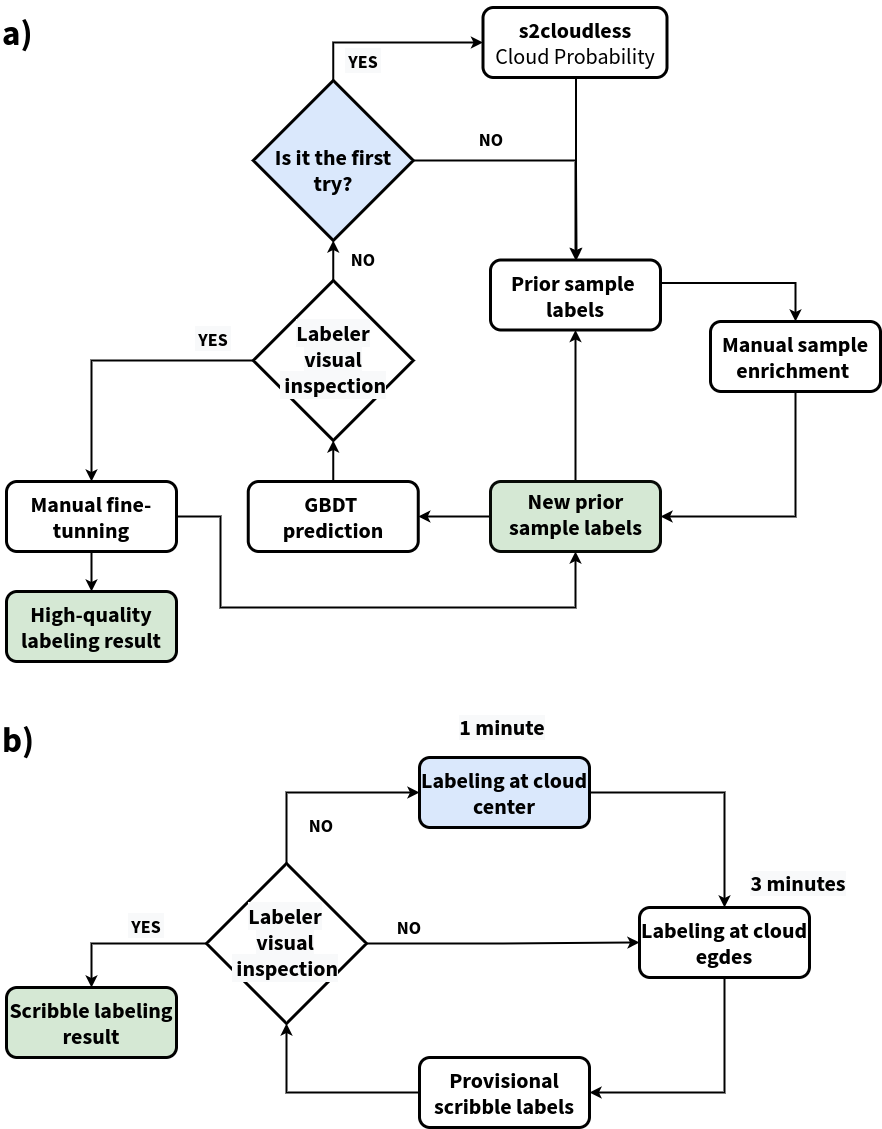
\includegraphics[width=0.98\linewidth]{figures/chapter01/figure07.png}
    \caption{a) High-quality labeling phase diagram. The model is set up using s2cloudless priors (blue). Annotations made by labelers with and without ML assistance are saved (green). b) Scribble labeling phase diagram. The labelers starts adding samples near to the centroids (blue), only the annotation cast by the labelers is preserved.}
    \label{fig:figure07}
\end{figure}

\hypertarget{quality-control-phase}{%
\subsection{Quality control phase}\label{quality-control-phase}}

Despite the human calibration phase, errors are still common in hand-operated labels. Therefore, statistic and visual inspections were implemented before admitting a manual annotation in CloudSEN12 (Figure \ref{fig:figure08}). First, an automatic check is set only for high-quality labels. It proposes that the GBDT accuracy during training must be higher than 0.95. This simple threshold pushes the CDE memsbers to set more samples and care more about labeling correctness. Later, two sequential visual inspection rounds are carried out for scribble and high-quality labels. The evaluators are two other CDE members than the one who labeled the IP. If a mistake is found, it is notified using GitHub Discussions\cite{Hata2022}. Finally, we discern the most challenging IPs (difficulty level greater than 4, see Table \ref{tab:table04}) and consult all CDE members to reaffirm or change a semantic class. The deliberations were supported by cloudApp (\href{https://csaybar.users.earthengine.app/view/cloudapp}{https://csaybar.users.earthengine.app/view/cloudapp}), which is a GEE web application that displays SEN2 image time series from any location on the earth (Figure \ref{fig:figureS02}).

\begin{figure}[!h]
    \centering
    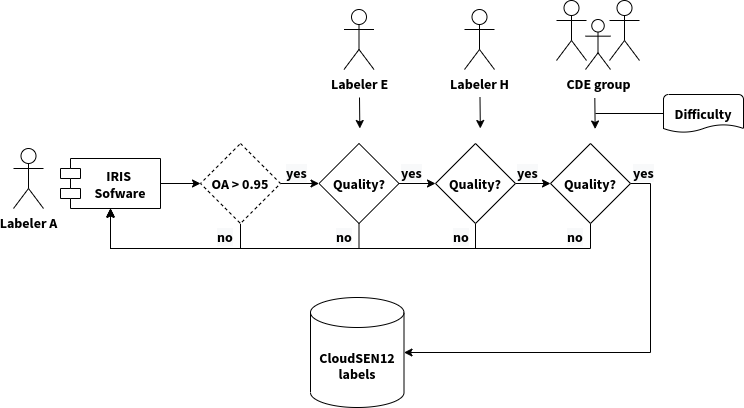
\includegraphics[width=0.98\linewidth]{figures/chapter01/figure08.png}
    \caption{Flowchart overview of the entire QC process.}
    \label{fig:figure08}
\end{figure}

\hypertarget{benchmarking-cloud-detection-models}{%
\subsection{Benchmarking cloud detection models}\label{benchmarking-cloud-detection-models}}

The variety of ways in which an EO model can be used makes benchmarking a difficult procedure\cite{CMIXRSE22}. For example, assessing CD model performance by seasonality rather than interannual or decadal variation may be more relevant in certain circumstances. Another example is that some data users may want to compare model performance geographically across different biomes or land-cover classes. A typical approach in EO is to benchmark models like traditional computer vision algorithms generating unique metrics for the entire datasets. However, this widespread practice can lead to biased conclusions. We argue that an appropriate model in EO must be capable of obtaining an adequate global metric while being consistent in space across multiple timescales. Furthermore, the observed patterns must be aligned with our physical understanding of the phenomena. In order to cover all the possible EO benchmarking user requirements, we added to each IP the results of eight of the most popular CD algorithms (see \textit{labels/} in Table\textasciitilde{}\ref{tab:table02}). This provides CloudSEN12 users more flexibility to choose a comparison strategy that is better tailored to their requirements. Next, we detail the CD algorithms available in CloudSEN12:

\begin{itemize}
    \item Fmask4: Function of Mask \cite{Qiu2019} cloud detection algorithm for Landsat and Sentinel-2. We use the MATLAB implementation code via Linux Docker containers \\ (\href{https://github.com/cloudsen12/models}{https://github.com/cloudsen12/models}.  We set the dilatation parameter for cloud, cloud shadow, and snow to 3, 3, and 0 pixels, respectively. The erosion radius (dilation) is set to 0 (90) meters, while the cloud probability threshold is fixed to 20\%.
    
    \item Sen2Cor: Software that performs atmospheric, terrain, and cirrus correction to SEN2 Level-1C input data. We store the Scene Classification (SC), which provides a semantic pixel-level classification map. The SC maps are obtained from the “COPERNICUS/S2\_SR” GEE dataset.
    
    \item s2cloudless: Single-scene CD algorithm created by Sentinel-Hub using a LightGBM decision tree model\cite{Ke2017}. The cloud probability values are collected without applying neither a threshold nor dilation. This resource is available in the “COPERNICUS/S2\_CLOUD\_PROBABILITY” GEE dataset.
    
    \item DL\_L8S2\_UV \cite{Lopez-Puigdollers2021}: U-Net with two different SEN2 band combinations: RGBI (B2, B3, B4, and B8) and RGBISWIR (B2, B3, B4, B8, B11, and B12) trained on the Landsat Biome-8 dataset (transfer learning\cite{MateoGarciaISPRS20,MateoGarciaJSTARS21} from Landsat 8 to Sentinel-2). 
    
    \item KappaMask \cite{Domnich2021}: U-Net with two distinct settings: all Sentinel-2 L1C bands and all Sentinel-2 L2A bands except the Red Edge 3 band. It was trained in an extension of the Sentinel-2 Cloud Mask Catalogue.
    
    \item QA60: Cloud mask embedded in the Quality assurance band of SEN2 Level-1C products.
\end{itemize}

Table\textasciitilde{}\ref{tab:table05} shows the cloud semantic categories for the different CD techniques available in CloudSEN12. It should be noted that only four CD algorithms provide the cloud shadow category.

\begin{table}[!h]
\centering
\caption{Output correspondence for different CD algorithms. Sen2Cor, Fmask, KappaMask, DL\_L8S2\_UV and S2cloudless are mapped respectively to CloudSEN12 cloud semantic categories. Adapted from Domnich et al.\cite{Domnich2021}}
\label{tab:table05}
\resizebox{\textwidth}{!}{%
\begin{tabular}{|l|l|l|l|l|l|l|}
\hline
\textbf{Sen2cor} & \textbf{KappaMask} & \textbf{CloudSEN12} & \textbf{Fmask} & \textbf{S2Cloudless} & \textbf{DL\_L8S2\_UV} & \textbf{QA60} \\ \hline
0 No data & 0 Missing & - &  &  &  &  \\ \hline
1 Saturated or defective &  & - &  &  &  &  \\ \hline
2 Dark area pixels &  & 0 Clear &  &  &  &  \\ \hline
3 Cloud shadows & 2 Cloud shadows & 3 Cloud shadows & 2 Cloud shadows &  &  &  \\ \hline
4 Vegetation & 1 Clear & 0 Clear & 0 Clear & 0 Clear & 0 Clear & 0 Clear \\ \hline
5 Bare Soils &  & 0 Clear &  &  &  &  \\ \hline
6 Water &  & 0 Clear & 1 Water &  &  &  \\ \hline
\begin{tabular}[c]{@{}l@{}}7 Cloud Low probability/\\ Unclassified\end{tabular} & 5 Undefined & - &  &  &  &  \\ \hline
8 Cloud medium probability &  & 1 Thick cloud &  &  &  &  \\ \hline
9 Cloud high probability &  & 1 Thick cloud & 4 Cloud & 1 Cloud & 1 Cloud & 1 Cloud \\ \hline
10 Thin cirrus & \begin{tabular}[c]{@{}l@{}}3 Semi-transparent \\ cloud\end{tabular} & 2 Thin cloud &  &  &  &  \\ \hline
11 Snow &  & 0 Clear & 3 Snow &  &  &  \\ \hline
\end{tabular}%
}
\end{table}

\hypertarget{preparing-cloudsen12-for-machine-learning}{%
\subsection{Preparing CloudSEN12 for machine learning}\label{preparing-cloudsen12-for-machine-learning}}

Splitting our densely annotated dataset into train and test sets is critical to ensure that ML practitioners are always using the same samples when providing results and to ensure that the tested algorithms provide a good generalization. Since cloud formation tends to fluctuate smoothly throughout space, a simple random split is suspicious to violate the assumption of test independence, especially under highly clustered labeled areas, such as the green and yellow regions shown in Figure\textasciitilde{}\ref{fig:figure01}. Therefore, we carry out a spatially stratified block split strategy\cite{Valavi2019}, based on Roberts et al.~2017 \cite{Roberts2017a}, to limit the risk of overfitting induced by spatial autocorrelation. First, we divided the Earth's surface into regular hexagons of 100 \(km^{2}\). Then, the initial hexagons are filtered, retaining only those that intersect with the high-quality dataset (Figure\textasciitilde{}\ref{fig:figure_S01}). Finally, using the difficulty IP property (see Table \ref{tab:table04}), we randomly stratified the remained blocks using 90\% (1827 ROIs) and 10\% (173 ROIs) for training and testing, respectively (Figure\textasciitilde{}\ref{fig:figure09}). The unlabeled and scribble datasets might be used as additional inputs for the training phase.

\begin{figure}[!h]
    \centering
    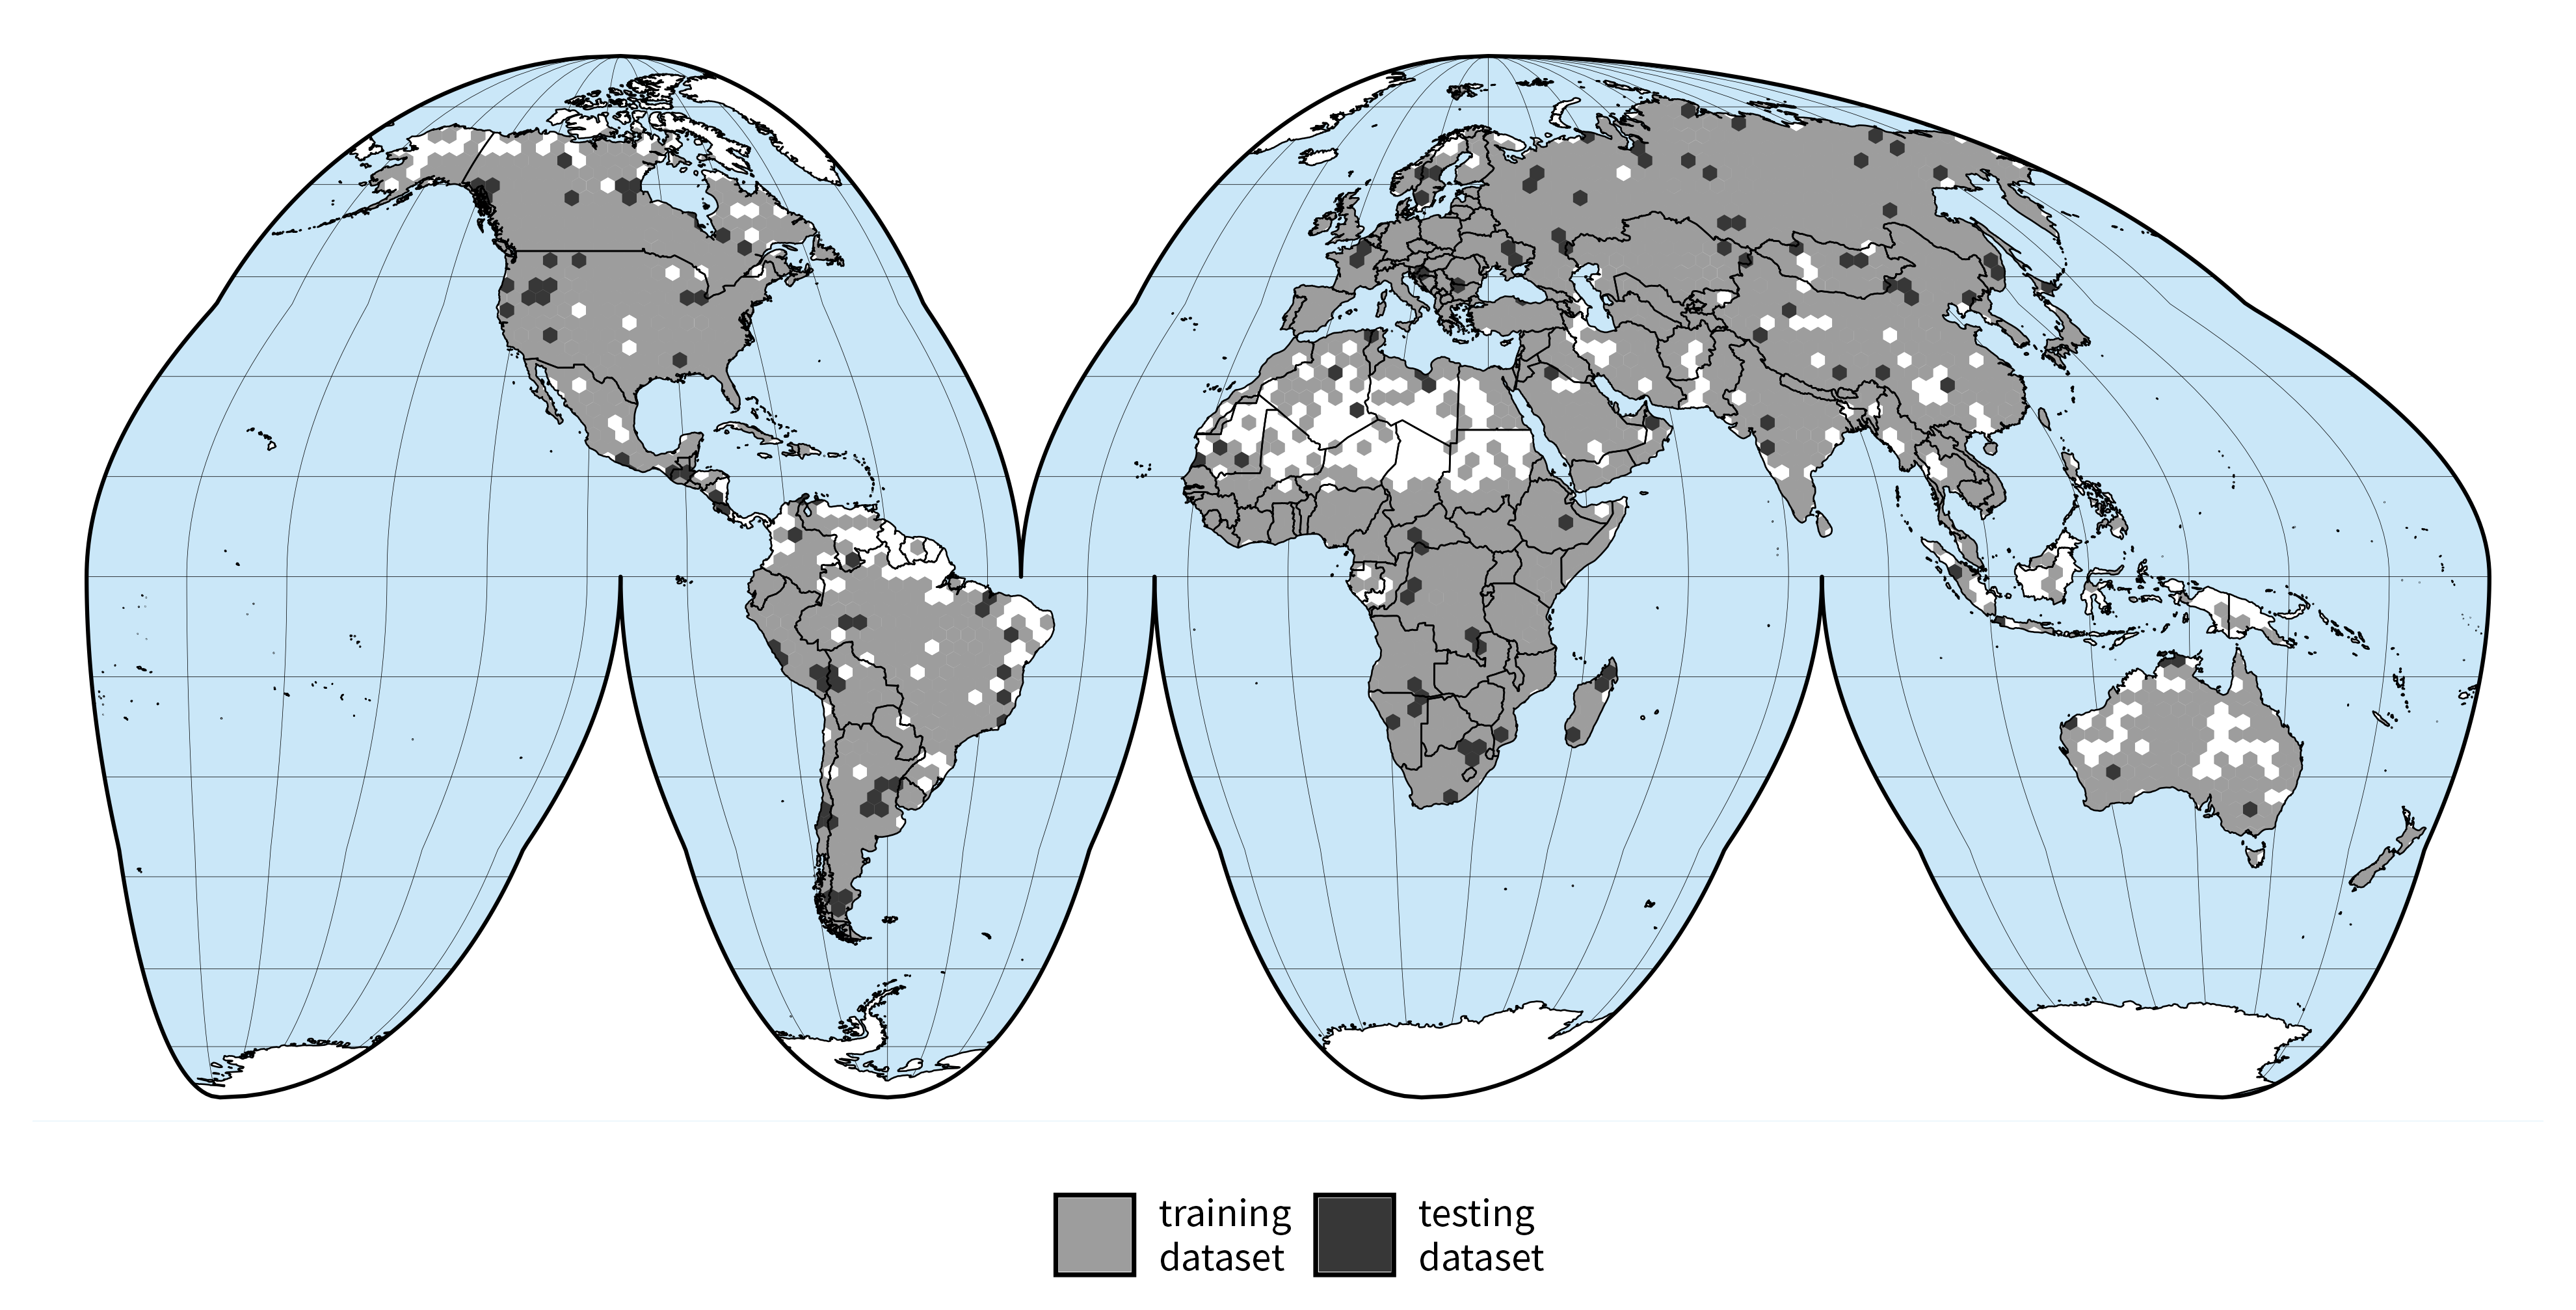
\includegraphics[width=0.9\linewidth]{figures/chapter01/figure09.png}
    \caption{Location of the training (blue) and testing (yellow) regions.}
    \label{fig:figure09}
\end{figure}

\hypertarget{data-record}{%
\section{Data Record}\label{data-record}}

The dataset is available via Radiant MLHub\cite{dsds} data repository at: \href{https://doi.org/10.34911/rdnt.y3xeg3}{https://doi.org/10.34911/rdnt.y3xeg3}. We defined an IP as the primary atomic unit, representing a single spatio-temporal component. Each IP has 49 assets (see Table \ref{tab:table02}) and 31 properties (see Table \ref{tab:table04}). All of the assets are delivered in the form of LZW-compressed COG (Cloud Optimized GeoTIFF) files. COG is an imagery format for web-optimized access to raster data that has a specific internal pixel structure that allows clients to request just specified areas of a large image by submitting HTTP range requests \cite{IosifescuEnescu2021}. The IP properties are shared using the SpatioTemporal Asset Catalog (STAC) specification. STAC provides a straightforward architecture for reading metadata and assets in JSON format, providing users with a sophisticated browsing experience that seamlessly integrates with modern scripting languages and front-end web technologies.

CloudSEN12 assets, as seen in Figure\textasciitilde{}\ref{fig:figure10}, are organized into four levels. The top-level includes three folders: high, scribble, and nolabel. These folders correspond to the annotation categories high-quality (2000 ROIs), scribble (2000 ROIs), and no annotation (5880 ROIs), respectively. In the second level, the folders included data pertaining to a given geographic location (ROI). The folder name is the ROI ID (Figure\textasciitilde{}\ref{fig:figure10}b). Since an ROI consists of five IPs at different dates, each ROI folder is subdivided into five folders whose names match the GEE Sentinel-2 product ID of the specific IP (Figure\textasciitilde{}\ref{fig:figure10}c). Finally, each IP folder stores the information detailed in Table\textasciitilde{}\ref{tab:table02} (Figure \ref{fig:figure10}d).

\hypertarget{technical-validation}{%
\section{Technical Validation}\label{technical-validation}}

This section reports CloudSEN12's suitability in multi-class semantic segmentation tasks. Based on Domnich et al.~\cite{Domnich2021} configuration, we trained a U-Net \cite{unet} model using all SEN2 L1C bands in the high-quality training dataset as input data. The high-quality test dataset (Figure \ref{fig:figure10}) is used to evaluate the algorithm performance by overall accuracy. A U-Net architecture is composed of three parts: (1) the encoder, which utilizes convolutional and max-pooling layers to extract features at multi-resolution level, (2) the bottleneck, that force to the model learns a compression of the input data, and (3) the decoder, which builds a segmentation map by combining the bottleneck results, deconvolutional layers for up-sampling and feature maps from the equivalent level in the encoder. In our U-Net implementation, we use MobileNetv2 \cite{Sandler2018} as encoder. The dice coefficient loss and the Adam optimizer are used for fitting the model. Besides, batch normalization layers are added after each convolutional layer for feature normalization throughout the network.

\hypertarget{usage-notes}{%
\section{Usage Notes}\label{usage-notes}}

This paper introduces CloudSEN12, a new large dataset for cloud semantic understanding, comprising 49,400 image patches distributed across all continents except Antarctica. The dataset has a total size of up to 1 TB. Nevertheless, we assume that most users experiments will only need a fraction of CloudSEN12. Therefore, to simplify its use, we developed a Python package called CloudSEN12. This Python package aims to help machine learning and remote sensing practitioners to:

\begin{itemize}
  \item Query and download the Radiant MLHub datasets using a user-friendly interface.
  \item Transform datasets to make them compatible with PyTorch DataLoader class.
  \item Provide pre-trained models based on the CloudSEN12 dataset.
\end{itemize}

The CloudSEN12 website \href{www.cloudsen12.github.io}{www.cloudsen12.github.io} includes tutorials for querying and downloading the dataset using the CloudSEN12 package. Besides, there are examples of how to train DL models using PyTorch. Finally, although CloudSEN12 was initially designed for semantic segmentation, it can be easily adapted to tackle other remote sensing problems like SAR-sharpening\cite{Schmitt2018a}, colorizing SAR images\cite{Schmitt2018b}, SAR-optical image matching\cite{Hughes2018}, and land cover mapping\cite{Karra2021}.

\hypertarget{code-availability}{%
\section{Code availability}\label{code-availability}}

The code to (1) create the raw CloudSEN12 imagery dataset, (2) download assets associated to each ROI, (3) create the manual annotations, (4) display cloudApp, (5) automatic perform cloud masking, (6) reproduce all the figures, (7) replicate the technical validation, (8) install CloudSEN12 Python package, and (9) deploy CloudSEN12 website is available in our Github organization \href{https://github.com/cloudsen12/}{https://github.com/cloudsen12/}.

\begin{savequote}
What am I in the eyes of most people - a nonentity, an eccentric or an
unpleasant person - somebody who has no position in society and never
will have, in short, the lowest of the low. All right, then - even if
that were absolutely true, then I should one day like to show by my work
what such an eccentric, such a nobody, has in his heart.
\qauthor{--- Vincent Van Gogh - 1882}\end{savequote}



\hypertarget{uncertainty-estimation}{%
\chapter{Uncertainty estimation}\label{uncertainty-estimation}}

\minitoc 

\hypertarget{introduction-1}{%
\section{Introduction}\label{introduction-1}}

Cloud masking is an essential pre-processing for any application of optical remote sensing imagery. Various coarse-resolution cloud cover datasets (\cite{sassen2008classifying, winker2010calipso, Wilson2016}) estimate the worldwide multi-annual cloud occurrence percentage to be around 0.6 ± 0.2, with hotspots in tropical and subtropical forests. Assuming these products are indicative of Sentinel-2 cloud conditions, we can anticipate that more than half of the pixels will need to be removed, i.e.~masked out, in order to avoid distortions in further analyses. Given that cloud masking can be interpreted as a statistical classification problem, the confusion matrix can be used to distinguish between two distinct types of errors. On the one hand, cloud omission errors (cloud as non-cloud) can lead to inconsistencies in time series of surface reflectance pixels, whereas cloud commission (clear as non-cloud) reduces the number of valid observations and, as a result, the frequency of cloud-free data (\cite{skakun2022cloud}). Cloud masking techniques are aimed to have a balance between commission and omission errors. Over the last three decades, a plethora of cloud masking methods have been presented (\cite{Hagolle2017, Domnich2021, Louis2016, Qiu2019, richter2019atmospheric, jan_wevers_2021_5788067, Lopez-Puigdollers2021, frantz2019force}). These methods can be classified into two main categories: knowledge-driven (KD) and data-driven (DD). While KD emphasizes the use of physical rules formulated on spectral and contextual features, DD is subjected to the exigency of large pixel-level annotation and costly computational requirements to distinguish cloud versus non-cloud regions.

Only a few studies have attempted to compare the various Sentinel-2 cloud masking methods. For instance, \cite{Cilli} compare DD with KD methods by analyzing 135 Sentinel-2 images distributed worldwide. They concluded that DD methods outperform KD methods. According to their experiments, \(10^{4}\) manually labeled pixels are sufficient for train machine learning algorithms to operate accurately cloud masking. Nonetheless, it is well established that DD models are highly dependent on the training dataset (\cite{Lopez-Puigdollers2021}). As a result, the comparison could be unfair, especially if the KD methods have not been as well calibrated to the dataset. \cite{Zekoll2021} compare three KD threshold-based: FMask, ATCOR, and Sen2Cor using a sample-based dataset. The results show that Sen2Cor outperforms the other methods. However, human-made datasets, especially those created by sampling, can be positively skewed if we consider that humans tend to overlook unpleasant information such as cloud borders (ostrich-effect, \cite{Valdez2017}). Using four different datasets, the Cloud Mask Intercomparison eXercise (CMIX) recently compared ten cloud detection algorithms. They suggested that no single algorithm performed better than the others (\cite{skakun2022cloud}). Similar conclusions are found in \cite{tarrio2020comparison} by analyzing 28 images over six Sentinel-2 tiles in Africa and Europe.

In this chapter, we propose to use a novel approach for
generating understanding
que nos permita predecir el error de sen2cor

cloud masking

exploiting the hand-crafted cloud and cloud shadow masking information freely available in cloudSEN12. Unlike previous studies, we intend not only to characterize but also to predict cloud masking uncertainty worldwide. Inspired by deep kernel learning \cite{wilson2016deep}, we explore the use of Gradient boosting Gaussian Processes (GBGP) which combines the structural properties of machine learning architectures with the non-parametric flexibility of kernel methods.

\hypertarget{data}{%
\section{Data}\label{data}}

The basis for Cmask is to predict what the reflectance would be for individual pixels in a Landsat 8 image if cirrus clouds were not present at the time the observations were collected. The basis for those pre- dictions is past observations and the atmospheric conditions, i.e.~the water vapor content, at the time of image acquisition. Therefore, two major inputs were included in this analysis: Integrated Water Vapor (IWV) provided by the second Modern-Era Retrospective analysis for Research and Applications (MERRA-2) and cirrus band time series provided by Landsat 8.

\hypertarget{cloudsen12}{%
\subsection{cloudSEN12}\label{cloudsen12}}

CloudSEN12 is a globally spatio-temporal distributed dataset for cloud and cloud shadow semantic understanding that consists of 49,400 image patches (IP) that are evenly spread throughout all continents except Antarctica (Figure X). Each IP has an average size of 5090 x 5090 meters and contains data from Sentinel-2 optical levels 1C and 2A, Sentinel-1 Synthetic Aperture Radar (SAR), digital elevation model, surface water occurrence, land cover classes, cloud masking results from eight different algorithms and hand-crafted labeling data created using an active learning system \cite{francis_alistair_2020_4172871}. cloudSEN12 offers three different manual annotation types in order to support different deep learning strategies: (i) 10,000 IPs with high-quality pixel-level annotation, (ii) 10,000 IPs with scribble annotation, and (iii) 29,250 unlabeled IPs. Only high-quality IPs are used in this study because of the risk of bias due scene incompleteness in scribble annotation. A detailed description of the CloudSEN12 dataset is given in chapter one.

\hypertarget{sen2cor}{%
\subsection{Sen2Cor}\label{sen2cor}}

Sentinel 2 Correction (\cite{Louis2016}) is a mono-temporal image processor designed for
scene classification and atmospheric correction of Sentinel-2 Level 1C input data. Sen2Cor version 2.8 is the version used in the Sentinel-2 ground segment with L2A processing baseline version 02.12. This processing baseline is the most recurrent version in cloudSEN12 (90\% IPs). Sen2Cor (Figure X) uses a series of spectral reflectance thresholds, ratios, and indices based on bands 1--5, 8, and 10--12 to compute cloud and snow probabilities for each pixel. Besides, it includes a cloud shadow and cirrus detection algorithm. The cloud shadows are estimated by multiplying two probability layers: (1) a geometric probability layer constructed from the
final thick cloud mask, sun position, and cloud height distribution, and (2) radiometric probability layer created from a Kohonen map to detect dark areas. On the other hand, cirrus probabilities are calculated simply by threshold band 10 (1.375 µm). Finally, a series of additional steps to improve the quality of the classification are automatically triggered using a priori information: digital elevation model (DEM) information, ESA CCI Water Bodies Map v4.0 (Lamarche et al., 2017), ESA CCI Land Cover Map v.2.0.7 (2015) and a snow climatology. In this study, SCL classes 8, 9 and 10 were used for cloud, class 3 for cloud shadow and the remaining SCL classes for non-cloud.

\hypertarget{cloud-type-ocurrence}{%
\subsection{Cloud type ocurrence}\label{cloud-type-ocurrence}}

The cloud type ocurrence (CTO) are derived from the CloudSat cloud profiling radar (CPR). This sensor permited for the first time to see cloud vertical structure (Stephens et al.~2008). ClouSat is part from Afternoon Constellation, or A-Train, at a frequency of 94 GHz and an altitude of about 700 km. Since 2011, it only produce daytime-only measurements due to battery malfunction, and in February 2018, the spacecraft systems moved to a lower orbit (C-train) to reduce the risk of collision with the other A-train spacecraft. The track of the satellite overpasses the same location every 16 days and provides a resolution of 1.4 km in cross-track and 1.8 km in along-track. Using the vertical profiles of clouds and precipitation, create an algorithms (\cite{}) to classify clouds according to the Cloud Climatology Project (ISCCP) approach: cumulus (Cu), stratocumulus (Sc), stratus (St), alto- cumulus (Ac), altostratus (As), nimbostratus (Ns), cirrus/ cirrostratus, or deep convective clouds. This information is storage in the 2B-CLDCLASS product. Particularly, in this study, we make use of the 3S-RMCP product of CloudSat level 3 observations. This product collocated 2B-CLDCLASS measurements in a 2.5°x2.5° grid. Based on this dataset, we constructed cloud type occurrence at 1° spatial
resolution. The TPR data used corresponds to the 2007--2016 period, the cloud type ocurrence were smoothed from 2.5° to 1° using cubic spline interpolation. We aggregathed the ISCCP classification into three classes accordin to the table x.

\hypertarget{modis}{%
\subsection{MODIS}\label{modis}}

\begin{table}[!h]
\resizebox{\textwidth}{!}{%
\begin{tabular}{|l|l|l|l|l|}
\hline
\multicolumn{1}{|c|}{\textbf{Dataset}} & \multicolumn{1}{c|}{\textbf{\begin{tabular}[c]{@{}c@{}}Used\\ for\end{tabular}}} & \multicolumn{1}{c|}{\textbf{\begin{tabular}[c]{@{}c@{}}Spatial \\ coverage\end{tabular}}} & \multicolumn{1}{c|}{\textbf{\begin{tabular}[c]{@{}c@{}}Data \\ Type\end{tabular}}} & \multicolumn{1}{c|}{\textbf{Description}} \\ \hline
Sen2Cor SLC - snow & T & Focal & B & \begin{tabular}[c]{@{}l@{}}Percentage of snow cover in a \\ cloudSEN12 IP.  If at least 5\% of snow\\ cover exists, 1; otherwise, 0.\end{tabular} \\ \hline
\begin{tabular}[c]{@{}l@{}}CloudSEN12 - cloud \\ type\end{tabular} & T & Focal & N & \begin{tabular}[c]{@{}l@{}}Metadata available in cloudSEN12,\\ derived from human-photo interpretation.\\ There are five classes: cumulus, stratus,\\ cirrus, haze, and contrails. A single IP \\ might have multiple classes.\end{tabular} \\ \hline
\begin{tabular}[c]{@{}l@{}}CloudSEN12 - cloud  \\ extent\end{tabular} & T & Focal & N & \begin{tabular}[c]{@{}l@{}}Metadata available in cloudSEN12, \\ derived from human-photo interpretation.\\ There are two classes: isolated, and\\ extended.\end{tabular} \\ \hline
\begin{tabular}[c]{@{}l@{}}CloudSAT 3S-RMCP -\\ cloud ocurrence\end{tabular} & P & Global & C & \begin{tabular}[c]{@{}l@{}}CloudSAT level 3 product used to \\ generalize CloudSEN12 - cloud \\ type in prediction time.\end{tabular} \\ \hline
\begin{tabular}[c]{@{}l@{}}CloudSEN12 -\\ Mean solar zenith \\ angle\end{tabular} & TP & Focal & C & \begin{tabular}[c]{@{}l@{}}The angle formed by the sun's beams \\ with respect to the vertical axis. In  \\ training phase values are obtained from \\ cloudSEN12 metadata. In prediction \\ phase is obtained by averaging image\\ properties from 2018 to 2020.\end{tabular} \\ \hline
\begin{tabular}[c]{@{}l@{}}MODIS - \\ MCD43A4.006\\ (HOT and NDVI)\end{tabular} & TP & Global & C & \begin{tabular}[c]{@{}l@{}}Spectral bands obtained from MODIS\\ composite from 2018 to 2020. In training\\ phase, the values are resampled considering\\ each specific cloudSEN12 IP geotransform. \\ Then, the pixels are spatially reduced \\ by the mean.\end{tabular} \\ \hline
\begin{tabular}[c]{@{}l@{}}MERIT Hydro - \\ Elevation\end{tabular} & TP & Global & C & Elevation map available in cloudSEN12. \\ \hline
\begin{tabular}[c]{@{}l@{}}Inter-annual\\ Cloud frecuency\end{tabular} & TP & Global & C & \multirow{2}{*}{Obtained from global 1-km cloud dataset.} \\ \cline{1-4}
\begin{tabular}[c]{@{}l@{}}Cloud intra-anual\\ variability\end{tabular} & TP & Global & C &  \\ \hline
Latitude & TP & Global & C & \multirow{2}{*}{\begin{tabular}[c]{@{}l@{}}In training phase are obtained from the\\ cloudSEN12 IP centroid.\end{tabular}} \\ \cline{1-4}
Longitude & TP & Global & C &  \\ \hline
\end{tabular}%
}
\end{table}

\hypertarget{methodology}{%
\section{Methodology}\label{methodology}}

This study aims to create a model that predicts cloud masking error in
a 1° x 1° worldwide grid system \(y^*\) from a set of predictors \(x^*\). The regression model \(\mathbf{f}\) is trained using a dataset, \(\mathcal{D} = \{x_i, y_i\}^{N}_{i=1}\) with \(x_i\) and \(y_i \in \mathbb{R}\). The segment \(x_i\) represents a vector of \(1 \times m\) predictors (Table X), \(y_i\) is the metric error values (see section \ref{section:metrics}) determined from comparing cloudSEN12 and Sen2Cor cloud masking results, and \(N\) the number of observations set as 10000. Only high-quality IPs are used in this study because of the risk of bias due to scene incompleteness in scribble annotation. A detailed description of the CloudSEN12 dataset is given in chapter one. We propose the use of a deep kernel learning (DKL) regression. It combines deep neural networks (DNN) with standard gaussian process regression (GP). While ANN captures the non-stationary and hierarchical structure, GP permits the estimation of their uncertainty considering the local autocorrelation of the observations. \cite{rasmussen2003gaussian} provide a detail description of GP. The standard GP, DKL, and the approach used to create worldwide cloud error predictions are briefly reviewed in the following sections.

\hypertarget{gaussian-process-regresion}{%
\subsection{Gaussian process regresion}\label{gaussian-process-regresion}}

Standard Gaussian Process Regression (GP) models is a expressive probabilistic model in which both training and testing data points are regarded samples of a joint multivariate normal distribution (\cite{williams2006gaussian}). As other regression models, a GP model is formed by noisy variables of the true underlying function \(\mathbf{f}\) that projects the vector space \(X\) into real-valued targets \(y\), i.e.~\(y = f(\mathbf{x}) + \epsilon\). The element \(\epsilon\) represents the noise variables with \(\mathcal{N}(0, \sigma^{2})\). In a GP model we assume that all the finite dimensional distributions \(f(\mathbf{x})\) are normally distributed with \(\mu\) as a mean and \(K_{XX}|\gamma\) as the prior covariance matrix. The covariance (kernel) matrix regulates the smoothness of GPs and its values are implicitly dependent on the kernel hyperparameters \(\gamma\). In this specific case, the estimation of \(f(\mathbf{x})\) can be expressed given by:

\begin{equation}
\begin{aligned}
\mathbf{f} = f(\mathbf{x}) = [f(x_1), ...., f(x_m)]^\top & \sim 
\mathcal{GP}\left(
  \mu, K_{XX}|\gamma\right
) \\
\end{aligned} \label{eq:1}
\end{equation}

Conditioning the joint normal distribution by the output values at the training points
(\(X\) and \(\mathbf{y}\)), the posterior distribution of the output values \(f(\mathbf{x}_{*})\) at the test data point \(X_*\) can be inferred as:

\begin{equation}
\begin{aligned}
f(\mathbf{x}_{*}) \mid X_{*}, X, \mathbf{y}, \boldsymbol{\gamma}, \sigma^{2} \sim \mathcal{N}(\mu^{*}, \Sigma^{*}), \\
\mu^{*} = \mu_{X_*} + K_{X_*X}\widehat{K}_{XX}^{-1}\mathbf{y}, \\
\Sigma^{*} = K_{X_*X_*} - K_{X_*X}\widehat{K}_{XX}^{-1}K_{XX_*}
\end{aligned} \label{eq:2}
\end{equation}

A hat denotes an added diagonal, i.e.~\(\widehat{K}_{XX} = K_{XX} + + \sigma^{2}I\). \(\mu^{*}\) and \(\Sigma^{*}\) are the posterior mean and covariance matrix respectively. The matrices of the form \(K_{X_iX_j}\) denote cross-covariances between the train (\(X\)) and test (\(X_*\)) vector spaces. The hyperparameters \(\lambda\) of the kernel are usually learned directly by minimizing the negative log marginal likelihood \(\mathcal{L}(\theta)\) with respect to training observations:

\begin{equation}
\begin{aligned}
\mathcal{L} = - \log p(\mathbf{y} \mid \gamma, X) \propto \mathbf{y}^{\top} \widehat{K}_{XX}^{-1} \mathbf{y} + \log \left|\widehat{K}_{X X}\right|, \\
\frac{\partial \mathcal{L}}{\partial \theta} = \mathbf{y}^{\top} \widehat{K}_{XX} \frac{\partial \widehat{K}_{X X}^{-1}}{\partial \theta} \widehat{K}_{X X} \mathbf{y}-\operatorname{tr}\left\{\widehat{K}_{X X}^{-1} \frac{\partial \widehat{K}_{XX}}{\partial \theta}\right\}
\label{eq:3}
\end{aligned}
\end{equation}

The main bottleneck for kernel learning is solve the linear system \(\widehat{K}_{XX}^{-1}y\) in equation \ref{eq:3}. The standard approach is to compute the Cholesky decomposition of the matrix \(\widehat{K}_{XX}^{-1}\). The Cholesky decomposition's core algorithm
uses a divide-and-conquer approach that is inefficient on GPU acceleration (\cite{krishnamoorthy2013matrix}). Furthermore, it requires \(\mathcal{O}(n^{3})\) computation and \(\mathcal{O}(n2)\) storage for GP inference and kernel learning (\cite{rasmussen2003gaussian}). To address the above challenges, several approaches to scaling up GP inference have been proposed (\cite{gardner2018gpytorch, cunningham2008fast, dong2017scalable, bach2013sharp, wilson2015thoughts}). In this paper, we address the GP inference issue by using the Blackbox Matrix-Matrix multiplication inference (BBMM, \cite{gardner2018gpytorch}). BBMM use preconditioned batched conjugate gradients to solve linear systems, reducing the asymptotic time complexity of GP inference from \(\mathcal{O}(n^{3})\) to \(\mathcal{O}(n^{2})\). Besides, it overcomes memory constraints by divvying the kernel matrix to perform matrix-vector multiplication (MVM, \cite{demmel1997applied}) without having to explicitly construct the kernel matrix, reducing the memory requirement to \(\mathcal{O}(n)\). Finally, BBMM parallelize partitioned MVMs across multiple core, enabling a better use of GPU hardware in comparison to the Cholesky factorization.

\hypertarget{deep-kernel-learning}{%
\subsection{Deep kernel learning}\label{deep-kernel-learning}}

DKL is a probabilistic deep network that simultaneously learns a feature
extractor and a Gaussian process on the feature space (cite). The network's
structure is depicted in Figure X. The deep non-linear feature extractor
\(\mathbf{h(x,w)}\), parametrized by weights \(\mathbf{w}\), is applied to the
observed input variable \(\mathbf{x}\). Next, the DNN outputs are modeled using
\(\mathcal{GP}\) by:

\begin{equation}
f(\mathbf{x}) \sim \mathcal{GP}(
    \mu(\mathbf{h_w(x)}),
    k_{\gamma}(\mathbf{h_w(x)}, \mathbf{h_w({x}')})
)
\end{equation}

All parameters of the model, including neural network weights \(\mathbf{w}\) and kernel parameters \(\mathbf{\gamma}\), are optimized end-to-end via backpropagation to minimize the negative log marginal likelihood (equation \ref{eq:3}).

\begin{figure}[!h]
    \centering
    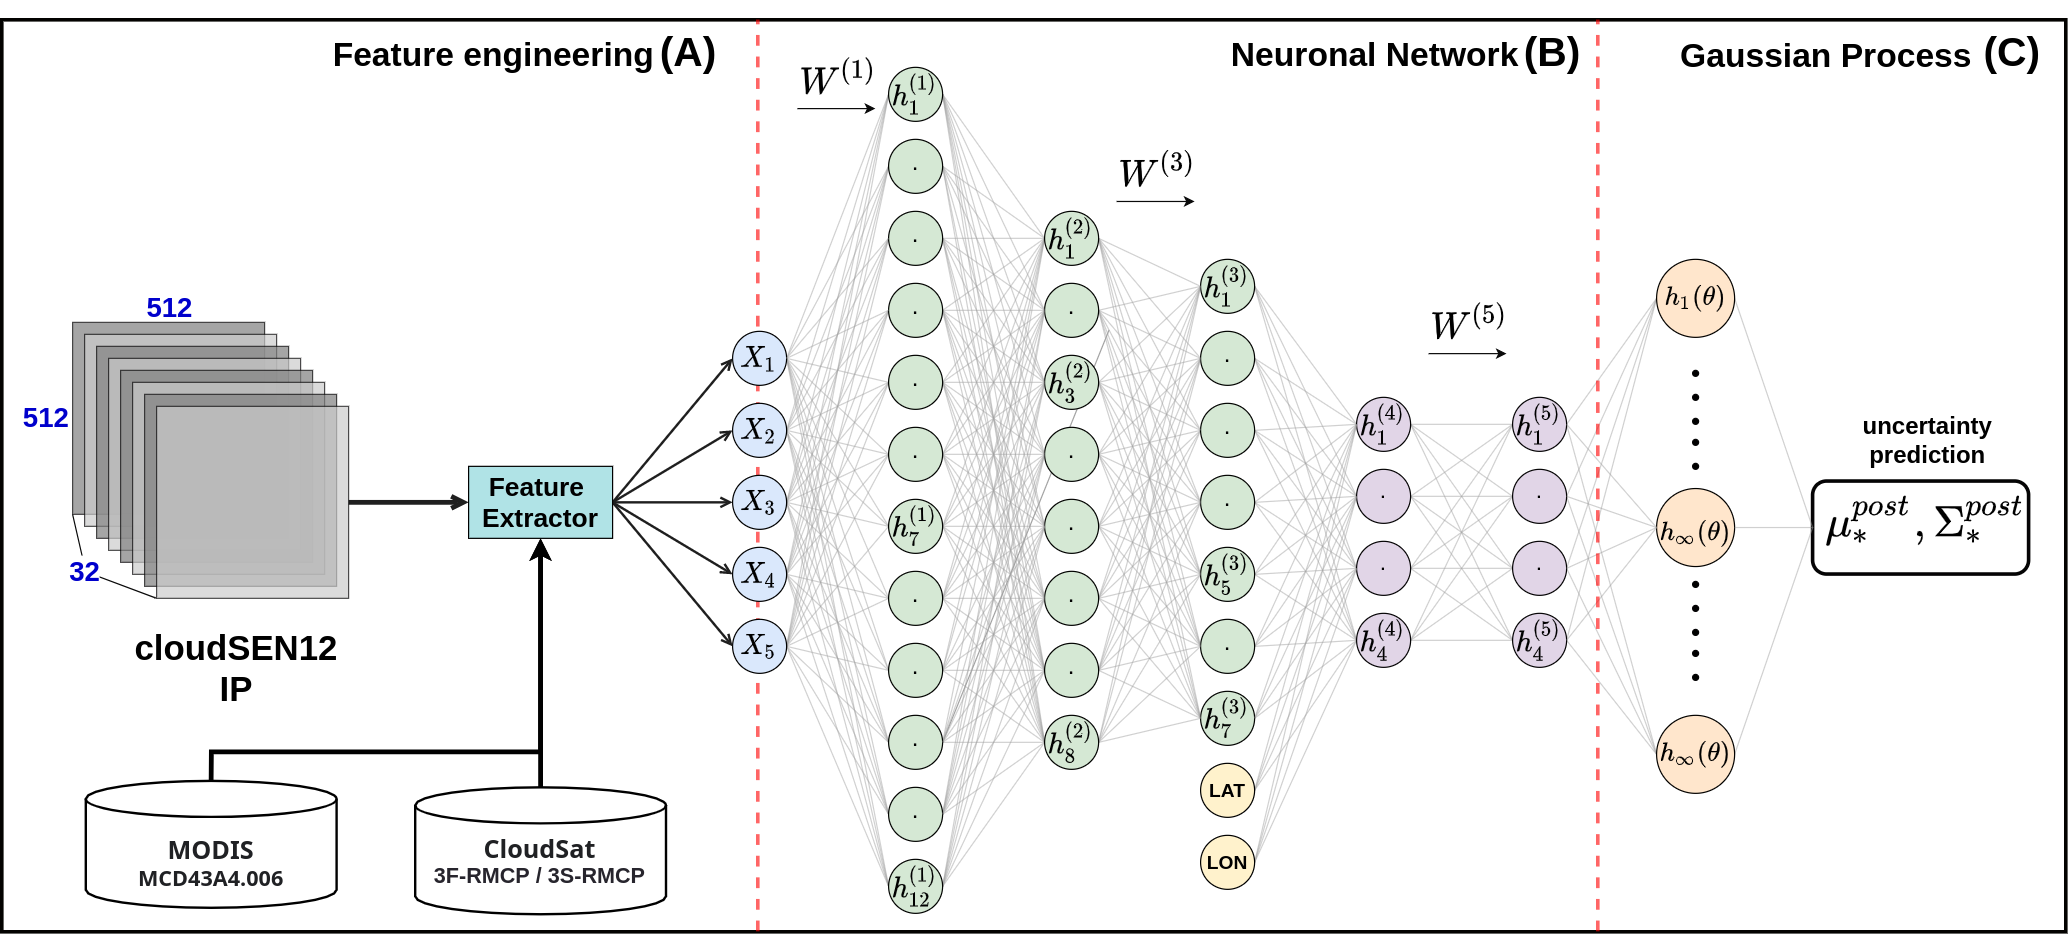
\includegraphics[width=1\linewidth]{figures/chapter02/figure02.png}
    \caption{Number of hand-crafted pixel annotations between different cloud detection datasets. All the labeled pixels in the CloudSEN12 no-annotation group come from cloud-free IPs.}
    \label{fig:figure02}
\end{figure}

\hypertarget{model-set-up-and-training}{%
\subsection{Model set-up and training}\label{model-set-up-and-training}}

For our deep kernel learning model, we used deep neural networks which produce
C-dimensional top-level features. Here C is the number of classes. We place a Gaussian process on each dimension of these features. We used RBF base kernels. The additive GP layer is then followed by a linear mixing layer A R C×C . We initialized A to be an identity matrix, and optimized in the joint learning procedure to recover cross-dimension correlations from data.
We first train a deep neural network using SGD with the softmax loss objective, and rectified linear activation functions. After the neural network has been pre-trained, we fit an additive KISS-GP layer, followed by a linear mixing layer, using the top-level features of the deep network as inputs. Using this pre-training initialization, our joint SV-DKL model of section 3 is then trained through the stochastic variational method of section 4 which jointly optimizes all the hyperparameters of the deep kernel (including all network weights), as well as the variational parameters, by backpropagating derivatives through the proposed marginal likelihood lower bound of the additive Gaussian process in section 4. In all experiments, we use a relatively large mini-batch size (specified according to the full data size), enabled by the proposed structure exploiting variational inference procedures. We achieve good performance setting the number of samples T = 1 in Eq. 4 for expectation estimation in variational inference, which provides additional confirmation for a similar observation in {[}14{]}.

\hypertarget{model-prediction}{%
\subsection{Model prediction}\label{model-prediction}}

\hypertarget{random-cross-validation}{%
\subsection{Random cross-validation}\label{random-cross-validation}}

\hypertarget{geographical-cross-validation}{%
\subsection{Geographical cross-validation}\label{geographical-cross-validation}}

\hypertarget{evaluation-metrics}{%
\subsection{Evaluation metrics}\label{evaluation-metrics}}

\label{section:metrics}

\hypertarget{experimental-results}{%
\section{Experimental results}\label{experimental-results}}

\hypertarget{discussion}{%
\section{Discussion}\label{discussion}}

dsada

\hypertarget{conclusion}{%
\section{Conclusion}\label{conclusion}}

dsada

\begin{savequote}
I may not have lived long, but I am certain of one thing. If there is a
type of person capable of changing something, it is someone who is
willing to sacrifice what he values most!. He is the type of person who,
in order to confront a monster, is capable of losing his own humanity. A
person who is unable to make a sacrifice may be unable to change
anything!
\qauthor{--- Armin Arlelt}\end{savequote}



\hypertarget{conclusion-1}{%
\chapter*{Conclusion}\label{conclusion-1}}
\addcontentsline{toc}{chapter}{Conclusion}

If we don't want Conclusion to have a chapter number next to it, we can add the \texttt{\{-\}} attribute.

\hypertarget{more-info}{%
\section*{More info}\label{more-info}}
\addcontentsline{toc}{section}{More info}

And here's some other random info:
the first paragraph after a chapter title or section head \emph{shouldn't be} indented, because indents are to tell the reader that you're starting a new paragraph.
Since that's obvious after a chapter or section title, proper typesetting doesn't add an indent there.

This paragraph, by contrast, \emph{will} be indented as it should because it is not the first one after the `More info' heading.
All hail LaTeX. (If you're reading the HTML version, you won't see any indentation - have a look at the PDF version to understand what in the earth this section is babbling on about).

\startappendices

\hypertarget{appendix---code}{%
\chapter{Appendix - Code}\label{appendix---code}}

This first appendix includes the non-stationary gaussian processes in Gpytorch:

\textbf{In 02-rmd-basics-code.Rmd}

\textbf{And here's another one from the same chapter, i.e.~Chapter \ref{code}:}

\hypertarget{appendix---figures}{%
\chapter{Appendix - Figures}\label{appendix---figures}}

\setcounter{figure}{0}
\makeatletter 
\renewcommand{\thefigure}{S\@arabic\c@figure}
\makeatother

\begin{figure}[!h]
    \centering
    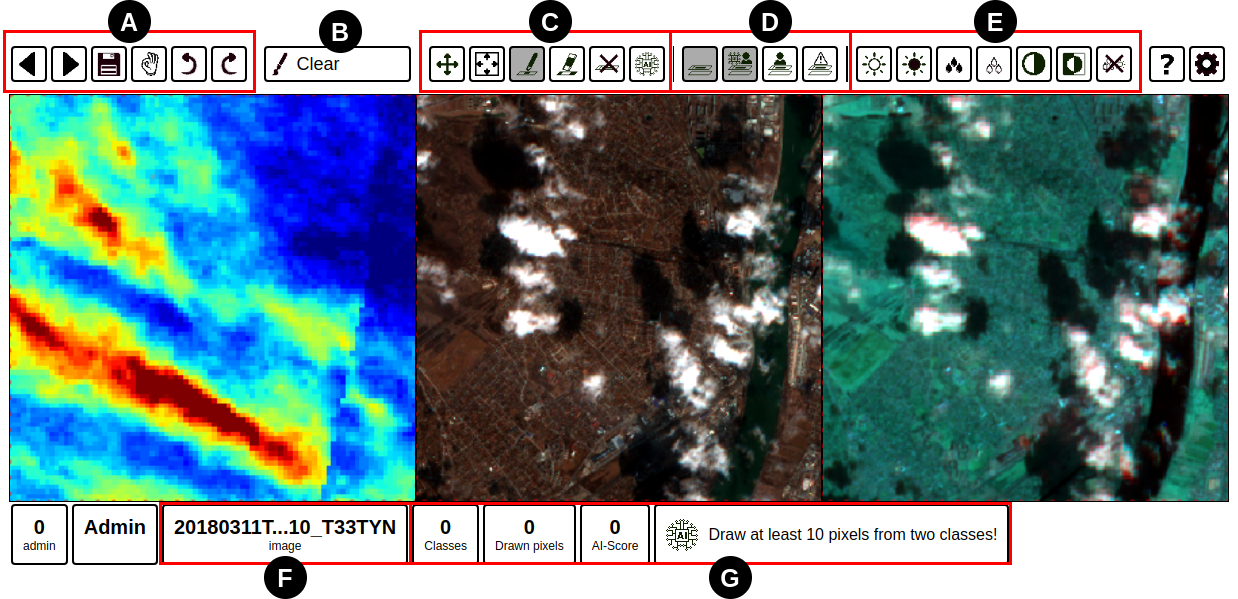
\includegraphics[width=1\linewidth]{figures/extra/figureS2.png}
    \caption{XXXX}
    \label{fig:figureS02}
\end{figure}

\begin{figure}[!h]
    \centering
    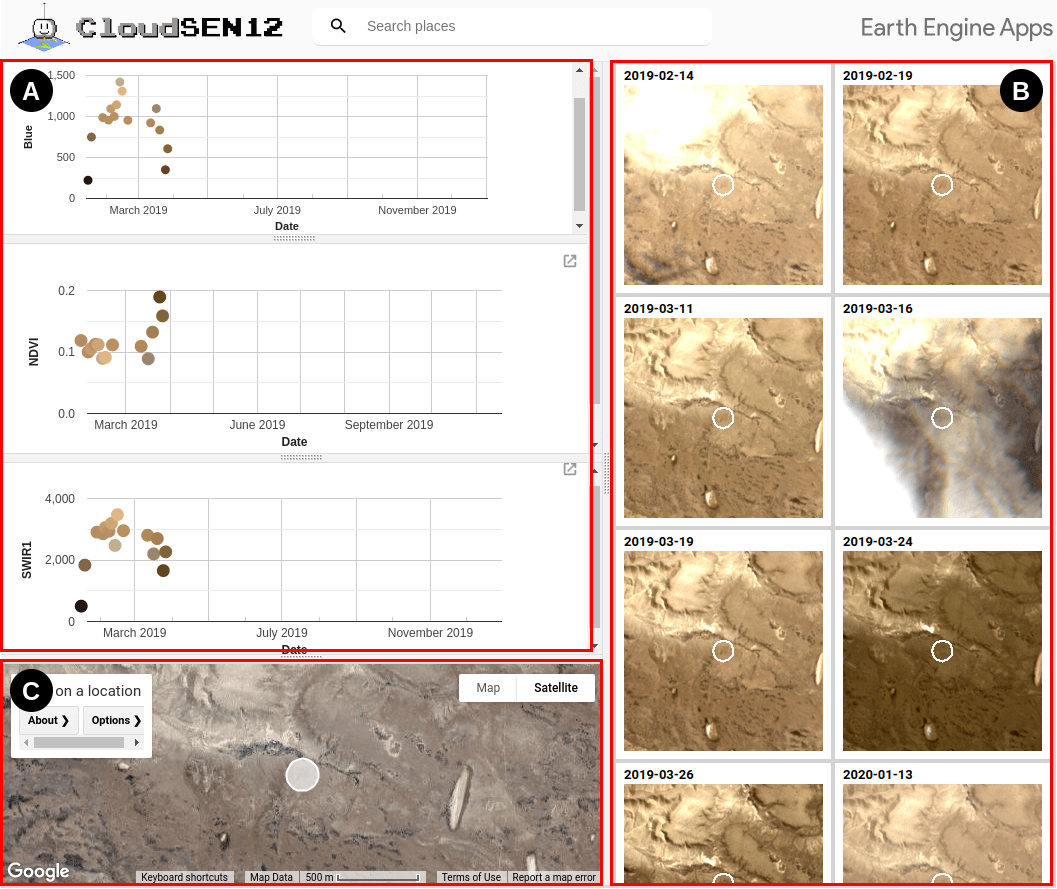
\includegraphics[width=1\linewidth]{figures/extra/figureS3.png}
    \caption{XXXX}
    \label{fig:figureS03}
\end{figure}


%%%%% REFERENCES
\setlength{\baselineskip}{0pt} % JEM: Single-space References

{\renewcommand*\MakeUppercase[1]{#1}%
\printbibliography[heading=bibintoc,title={\bibtitle}]}


\end{document}
